\documentclass[12pt, a4paper]{article}

\usepackage{amsmath}
\usepackage{amsfonts}
\usepackage{amssymb}
\usepackage{graphicx}
\usepackage{float}
\usepackage{listings}
\usepackage{rotating}
\usepackage{tikz}
\pdfgentounicode=1
\pdfmapline{+cyberb@Unicode@  <cyberbit.ttf}

\begin{document}

\title{SpringSys}
\author{P. Baillehache}
\date{\today}
\maketitle

\tableofcontents

\section*{Introduction}

SpringSys is a C library to simulate systems of masses connected by springs.\\

The number of dimensions of the system can be 1,2 or 3. It has a dissipation coefficient used to simulate dissipation of energy and dampen the system behaviour. A mass is defined by its mass, position and speed. A spring is defined by its rigidity coefficient, length (min, max, current and at rest), and the 2 masses it connects. A spring an be unbreakable or breakable (under stress limit condition).\\

SpringSys offers functions to create the system by adding/removing masses and springs or by cloning another SpringSys, to step in time the system, to step it until it reach equilibrium, to print it, to get the total stress and momentum of the system, to load ans save the system to a text file, to get the nearest mass or spring to a given position.\\ 

\section{Interface}

\begin{scriptsize}
\begin{ttfamily}
\begin{lstlisting}
// ============ SPRINGSYS.H ================

#ifndef SPRINGSYS_H
#define SPRINGSYS_H

// ================= Include =================

#include <stdlib.h>
#include <stdio.h>
#include <math.h>
#include <string.h>
#include <stdbool.h>
#include "gset.h"

// ================= Define ==================

#define SPRINGSYS_EPSILON 0.0000001

// ================= Data structure ===================

typedef struct SpringSysMass {
  // ID
  int _id;
  // Position
  float _pos[3];
  // Speed
  float _speed[3];
  // Stress (acceleration due to the springs)
  float _stress[3];
  // Mass 
  float _mass;
  // Fixed flag, if true the mass doesn't move
  bool _fixed;
} SpringSysMass;

typedef struct SpringSysSpring {
  // ID
  int _id;
  // Current length
  float _length;
  // K coefficient
  float _k;
  // Length at rest
  float _restLength;
  // Stress (positive = extension, negative = compression)
  float _stress;
  // Limit stress (compression/extension)
  // If the current stress get over the limits the spring breaks (it
  // is removed from the list of springs)
  float _maxStress[2];
  // ID of the masses at the extremities of the spring
  int _mass[2];
  // Breakable flag, if true the spring breaks if its stress goes over 
  // the limit _maxStress
  bool _breakable;
} SpringSysSpring;

typedef struct SpringSys {
  // List of masses
  GSet *_masses;
  // List of springs
  GSet *_springs;
  // Number of dimension of the system (in [1, 3])
  int _nbDim;
  // Dissipation coefficient (applied to speed of masses at each step,
  // 0.0 = no dissipation, 1.0 = total dissipation)
  float _dissip;
} SpringSys;

// ================ Functions declaration ====================

// Create a new SpringSys with number of dimensions 'nbDim' (in [1,3])
// Default dissipation coefficient _dissip = 0.01
// Return NULL if we couldn't create the Springsys
SpringSys* SpringSysCreate(int nbDim);

// Clone the SpringSys 'sys'
// Return NULL if we couldn't clone the Springsys
SpringSys* SpringSysClone(SpringSys *sys);

// Load the SpringSys 'sys' from the stream 'stream'
// If 'sys' is already allocated, it is freed before loading
// Return 0 in case of success, or:
// 1: invalid arguments
// 2: can't allocate memory
// 3: invalid data
int SpringSysLoad(SpringSys **sys, FILE *stream);

// Save the SpringSys 'sys' to the stream
// Return 0 upon success, else
int SpringSysSave(SpringSys *sys, FILE *stream);

// Create a default mass, default properties' values are:
// _id = 0;
// _pos[0] = _pos[1] = _pos[2] = 0.0;
// _nextPos[0] = _nextPos[1] = _nextPos[2] = 0.0;
// _speed[0] = _speed[1] = _speed[2] = 0.0;
// _stress[0] = _stress[1] = _stress[2] = 0.0;
// _mass = 1.0;
// _fixed = false;
// Return NULL if memory allocation failed
SpringSysMass* SpringSysCreateMass(void);

// Create a default spring, default properties' values are:
// _id = 0;
// _length = 1.0;
// _k = 1.0;
// _restLength = 1.0;
// _stress = 0.0;
// _maxLength[0] = 0.0;
// _maxLength[1] = 100.0;
// _maxStress[0] = -1000000.0;
// _maxStress[1] = 1000000.0;
// _mass[0] = 0;
// _mass[1] = 0;
// _breakable = false
// Return NULL if memory allocation failed
SpringSysSpring* SpringSysCreateSpring(void);

// Free the memory used by a SpringSys
// Do nothing if arguments are invalid
void SpringSysFree(SpringSys **sys);

// Free the memory used by a SpringSysMass
// Do nothing if arguments are invalid
void SpringSysMassFree(SpringSysMass **m);

// Free the memory used by a SpringSysSpring
// Do nothing if arguments are invalid
void SpringSysSpringFree(SpringSysSpring **s);

// Print the SpringSys on 'stream'
// Do nothing if arguments are invalid
void SpringSysPrint(SpringSys *sys, FILE *stream);

// Print the SpringSysMass on 'stream'
// Do nothing if arguments are invalid
void SpringSysMassPrint(void *m, FILE *stream);

// Print the SpringSysSpring on 'stream'
// Do nothing if arguments are invalid
void SpringSysSpringPrint(void *s, FILE *stream);

// Set the dissipation coefficient of the SpringSys to 'dissip' 
// in [0.0,1.0]
// Do nothing if arguments are invalid
void SpringSysSetDissip(SpringSys *sys, float dissip);

// Get the mass identified by 'id'
// Return NULL if arguments are invalid or if there is no mass 
// with this id
SpringSysMass* SpringSysGetMass(SpringSys *sys, int id);

// Get the spring identified by 'id'
// Return NULL if arguments are invalid or if there is no spring 
// with this id
SpringSysSpring* SpringSysGetSpring(SpringSys *sys, int id);

// Get the number of mass in the SpringSys
// Return -1 if the argument are invalid
int SpringSysGetNbMass(SpringSys *sys);

// Get the number of spring in the SpringSys
// Return -1 if the argument are invalid
int SpringSysGetNbSpring(SpringSys *sys);

// Add a copy of the mass 'm' to the SpringSys
// Return false if the arguments are invalid or memory allocation failed
// else return true
bool SpringSysAddMass(SpringSys *sys, SpringSysMass *m);

// Add a copy of the spring 's' to the SpringSys
// Return false if the arguments are invalid or memory allocation failed
// else return true
bool SpringSysAddSpring(SpringSys *sys, SpringSysSpring *s);

// Remove the mass identified by 'id'
// Springs connected to this mass are removed as well
// Do nothing if arguments are invalids
void SpringSysRemoveMass(SpringSys *sys, int id);

// Remove spring idenitfied by 'id'
// Do nothing if argument are invalids
void SpringSysRemoveSpring(SpringSys *sys, int id);

// Step in time by 'dt' the SpringSys
// 'dt' must be carefully choosen, if too big inaccuracy of the 
// simulation leads to divergence and then to rupture of springs,
// especially if springs have a high mk coefficient 
// Do nothing if arguments are invalid
void SpringSysStep(SpringSys *sys, float dt);

// Step in time by 'dt' the SpringSys until it is in equilibrium 
// or 'tMax' has been reached
// 'dt' must be carefully choosen, if too big inaccuracy of the 
// simulation leads to divergence and then to rupture of springs,
// especially if springs have a high mk coefficient 
// Return a value > tMax if the arguments are invalid or the equilibrium
// couldn't be reached, else return the time it took to 
// reach equilibrium 
float SpringSysStepToRest(SpringSys *sys, float dt, float tMax);

// Get the momentum (sum of norm(v) of masses) of the SpringSys
// Return 0.0 if the arguments are invalid
float SpringSysGetMomentum(SpringSys *sys);

// Get the stress (sum of abs(stress) of springs) of the SpringSys
// Return 0.0 if the arguments are invalid
float SpringSysGetStress(SpringSys *sys);

// Get the nearest mass to 'pos' in the SpringSys 'sys'
// Return NULL if arguments are invalids
SpringSysMass* SpringSysGetMassByPos(SpringSys *sys, float *pos);

// Get the nearest spring to 'pos' in the SpringSys 'sys'
// Return NULL if arguments are invalids
SpringSysSpring* SpringSysGetSpringByPos(SpringSys *sys, float *pos);

#endif
\end{lstlisting}
\end{ttfamily}
\end{scriptsize}

\section{Code}

\begin{scriptsize}
\begin{ttfamily}
\begin{lstlisting}
// ============ SPRINGSYS.C ================

#include "springsys.h"

// ================= Include =================

// Create a new SpringSys with number of dimensions 'nbDim' (in [1,3])
// Default dissipation coefficient _dissip = 0.01
// Return NULL if we couldn't create the Springsys
SpringSys* SpringSysCreate(int nbDim) {
  // Check arguments
  if (nbDim < 1 || nbDim > 3)
    return NULL;
  // Allocate memory for the new SpringSys
  SpringSys *ret = (SpringSys*)malloc(sizeof(SpringSys));
  // If we could allocate memory
  if (ret != NULL) {
    // Set the number of dimensions
    ret->_nbDim = nbDim;
    // Set the dissipation coefficient
    ret->_dissip = 0.01;
    // Create the gset of masses
    ret->_masses = GSetCreate();
    // If we couldn't create the gset
    if (ret->_masses == NULL) {
      // Free memory
      free(ret);
      // Return NULL
      return NULL;
    }
    // Create the gset of springs
    ret->_springs = GSetCreate();
    // If we couldn't create the gset
    if (ret->_springs == NULL) {
      // Free memory
      GSetFree(&(ret->_masses));
      free(ret);
      // Return NULL
      return NULL;
    }
  }
  return ret;
}

// Clone the SpringSys 'sys'
// Return NULL if we couldn't clone the Springsys
SpringSys* SpringSysClone(SpringSys *sys) {
  // Check arguments
  if (sys == NULL)
    return NULL;
  // Allocate memory for the new SpringSys
  SpringSys *ret = (SpringSys*)malloc(sizeof(SpringSys));
  // If we could allocate memory
  if (ret != NULL) {
    // Set the number of dimensions
    ret->_nbDim = sys->_nbDim;
    // Set the dissipation coefficient
    ret->_dissip = sys->_dissip;
    // Initialize the pointer to gsets of masses and springs
    ret->_masses = NULL;
    ret->_springs = NULL;
    // Create the gset of masses
    ret->_masses = GSetCreate();
    // If we couldn't create the gset
    if (ret->_masses == NULL) {
      // Free memory
      free(ret);
      // Return NULL
      return NULL;
    }
    // Create the gset of springs
    ret->_springs = GSetCreate();
    // If we couldn't create the gset
    if (ret->_springs == NULL) {
      // Free memory
      GSetFree(&(ret->_masses));
      free(ret);
      // Return NULL
      return NULL;
    }
    // If there is a gset of masses
    if (sys->_masses != NULL) {
      // Copy the masses
      GSetElem *m = sys->_masses->_head;
      while (m != NULL) {
        // Declare a variable to create the clone of the mass
        SpringSysMass *mass = NULL;
        // If the mass is not null in the SpringSys
        if (m->_data != NULL) {
          // Allocate memory for the clone of the mass
          mass = (SpringSysMass*)malloc(sizeof(SpringSysMass));
          // If we couldn't allocate memory
          if (mass == NULL) {
            // Free the memory
            SpringSysFree(&ret);
            // Return NULL
            return NULL;
          }
          // Clone the mass
          memcpy(mass, m->_data, sizeof(SpringSysMass));
        }
        // Get the current number of masses
        int nbMass = ret->_masses->_nbElem;
        // Append the mass
        GSetAppend(ret->_masses, mass);
        // If we couldn't append the mass
        if (nbMass + 1 != ret->_masses->_nbElem) {
          // Free the memory
          free(mass);
          SpringSysFree(&ret);
          // Return NULL
          return NULL;
        }
        // Move to the next element
        m = m->_next;
      }
    }
    // If there is a gset of springs
    if (sys->_springs != NULL) {
      // Copy the springs
      GSetElem *s = sys->_springs->_head;
      while (s != NULL) {
        // Declare a variable to create the clone of the spring
        SpringSysSpring *spring = NULL;
        // If the spring is not null in the SpringSys
        if (s->_data != NULL) {
          // Allocate memory for the clone of the spring
          spring = (SpringSysSpring*)malloc(sizeof(SpringSysSpring));
          // If we couldn't allocate memory
          if (spring == NULL) {
            // Free the memory
            SpringSysFree(&ret);
            // Return NULL
            return NULL;
          }
          // Clone the spring
          memcpy(spring, s->_data, sizeof(SpringSysSpring));
        }
        // Get the current number of springs
        int nbSpring = ret->_springs->_nbElem;
        // Append the spring
        GSetAppend(ret->_springs, spring);
        // If we couldn't append the spring
        if (nbSpring + 1 != ret->_springs->_nbElem) {
          // Free the memory
          free(spring);
          SpringSysFree(&ret);
          // Return NULL
          return NULL;
        }
        // Move to the next element
        s = s->_next;
      }
    }
  }
  return ret;
}

// Load the SpringSys 'sys' from the stream 'stream'
// If 'sys' is already allocated, it is freed before loading
// Return 0 in case of success, or:
// 1: invalid arguments
// 2: can't allocate memory
// 3: invalid data
int SpringSysLoad(SpringSys **sys, FILE *stream) {
  // Check arguments
  if (sys == NULL || stream == NULL)
    return 1;
  // If the SpringSys is already allocated
  if (*sys != NULL)
    // Free memory
    SpringSysFree(sys);
  // Read the number of dimension
  int nbDim;
  int ret = fscanf(stream, "%d\n", &nbDim);
  // Allocate memory for the SpringSys
  *sys = SpringSysCreate(nbDim);
  // If we couldn't allocate memory
  if (*sys == NULL)
    // Stop here
    return 2;
  // Create a mass to read the data
  SpringSysMass *mass = SpringSysCreateMass();
  if (mass == NULL) {
    SpringSysFree(sys);
    return 2;
  }
  // Create a spring to read the data
  SpringSysSpring *spring = SpringSysCreateSpring();
  if (spring == NULL) {
    SpringSysMassFree(&mass);
    SpringSysFree(sys);
    return 2;
  }
  // Read the number of mass
  int nbMass;
  ret = fscanf(stream, "%d\n", &nbMass);
  // For each mass
  for (int iMass = 0; iMass < nbMass; ++iMass) {
    // Read the properties of the mass
    ret = fscanf(stream, "%d\n", &(mass->_id));
    ret = fscanf(stream, "%f %f %f\n", &(mass->_pos[0]), 
      &(mass->_pos[1]), &(mass->_pos[2]));
    ret = fscanf(stream, "%f %f %f\n", &(mass->_speed[0]), 
      &(mass->_speed[1]), &(mass->_speed[2]));
    ret = fscanf(stream, "%f %f %f\n", &(mass->_stress[0]), 
      &(mass->_stress[1]), &(mass->_stress[2]));
    ret = fscanf(stream, "%f\n", &(mass->_mass));
    int b;
    ret = fscanf(stream, "%d\n", &b);
    mass->_fixed = b;
    // Add the mass
    bool ok = SpringSysAddMass(*sys, mass);
    // If we couldn't add the mass
    if (ok == false) {
      SpringSysMassFree(&mass);
      SpringSysSpringFree(&spring);
      SpringSysFree(sys);
      return 3;
    }
  }
  // Read the number of spring
  int nbSpring;
  ret = fscanf(stream, "%d\n", &nbSpring);
  // For each spring
  for (int iSpring = 0; iSpring < nbSpring; ++iSpring) {
    // Read the properties of the spring
    ret = fscanf(stream, "%d\n", &(spring->_id));
    ret = fscanf(stream, "%f\n", &(spring->_length));
    ret = fscanf(stream, "%f\n", &(spring->_k));
    ret = fscanf(stream, "%f\n", &(spring->_restLength));
    ret = fscanf(stream, "%f\n", &(spring->_stress));
    ret = fscanf(stream, "%f %f\n", &(spring->_maxStress[0]), 
      &(spring->_maxStress[1]));
    ret = fscanf(stream, "%d %d\n", &(spring->_mass[0]), 
      &(spring->_mass[1]));
    int b;
    ret = fscanf(stream, "%d\n", &b);
    spring->_breakable = b;
    // Add the spring
    bool ok = SpringSysAddSpring(*sys, spring);
    // If we couldn't add the spring
    if (ok == false) {
      SpringSysMassFree(&mass);
      SpringSysSpringFree(&spring);
      SpringSysFree(sys);
      return 3;
    }
  }
  // TODO don't ignore the return value
  ret = ret;
  // Free memory
  SpringSysMassFree(&mass);
  SpringSysSpringFree(&spring);
  // Return success code
  return 0;
}

// Save the SpringSys 'sys' to the stream
// Return 0 upon success, else
// 1: invalid argument
// 2: invalid SpringSys
int SpringSysSave(SpringSys *sys, FILE *stream) {
  // Check arguments
  if (sys == NULL || sys->_masses == NULL || 
    sys->_springs == NULL || stream == NULL)
    return 1;
  // Write the number of dimensions
  fprintf(stream, "%d\n", sys->_nbDim);
  // Write the number of masses
  fprintf(stream, "%d\n", sys->_masses->_nbElem);
  // Get a pointer to the first element of the list of masses
  GSetElem *e = sys->_masses->_head;
  // While we are not at the end of the list
  while (e != NULL) {
    // Get a pointer to the mass
    SpringSysMass *m = (SpringSysMass*)(e->_data);
    // If the pointer is not null
    if (m != NULL) {
      // Write the mass properties
      fprintf(stream, "%d\n", m->_id);
      fprintf(stream, "%f %f %f\n", m->_pos[0], m->_pos[1], m->_pos[2]);
      fprintf(stream, "%f %f %f\n", m->_speed[0], m->_speed[1], 
        m->_speed[2]);
      fprintf(stream, "%f %f %f\n", m->_stress[0], m->_stress[1], 
        m->_stress[2]);
      fprintf(stream, "%f\n", m->_mass);
      fprintf(stream, "%d\n", m->_fixed);
    // Else, the pointer is null
    } else {
      // This should never happen
      return 2;
    }
    // Move to the next element
    e = e->_next;
  }
  // Write the number of springs
  fprintf(stream, "%d\n", sys->_springs->_nbElem);
  // Get a pointer to the first element of the list of springs
  e = sys->_springs->_head;
  // While we are not at the end of the list
  while (e != NULL) {
    // Get a pointer to the spring
    SpringSysSpring *s = (SpringSysSpring*)(e->_data);
    // If the pointer is not null
    if (s != NULL) {
      // Write the spring properties
      fprintf(stream, "%d\n", s->_id);
      fprintf(stream, "%f\n", s->_length);
      fprintf(stream, "%f\n", s->_k);
      fprintf(stream, "%f\n", s->_restLength);
      fprintf(stream, "%f\n", s->_stress);
      fprintf(stream, "%f %f\n", s->_maxStress[0], s->_maxStress[1]);
      fprintf(stream, "%d %d\n", s->_mass[0], s->_mass[1]);
      fprintf(stream, "%d\n", s->_breakable);
    // Else, the pointer is null
    } else {
      // This should never happen
      return 2;
    }
    // Move to the next element
    e = e->_next;
  }
  return 0;
}

// Create a default mass
// Return NULL if memory allocation failed
SpringSysMass* SpringSysCreateMass(void) {
  // Allocate memory
  SpringSysMass *ret = (SpringSysMass*)malloc(sizeof(SpringSysMass));
  // If we could allocate memory
  if (ret != NULL) {
    // Set default values for the properties
    ret->_id = 0;
    ret->_pos[0] = ret->_pos[1] = ret->_pos[2] = 0.0;
    ret->_speed[0] = ret->_speed[1] = ret->_speed[2] = 0.0;
    ret->_stress[0] = ret->_stress[1] = ret->_stress[2] = 0.0;
    ret->_mass = 1.0;
    ret->_fixed = false;
  }
  // Return the new mass
  return ret;
}

// Create a default spring
// Return NULL if memory allocation failed
SpringSysSpring* SpringSysCreateSpring(void) {
  // Allocate memory
  SpringSysSpring *ret = 
    (SpringSysSpring*)malloc(sizeof(SpringSysSpring));
  // If we could allocate memory
  if (ret != NULL) {
    // Set default values for the properties
    ret->_id = 0;
    ret->_length = 1.0;
    ret->_k = 1.0;
    ret->_restLength = 1.0;
    ret->_stress = 0.0;
    ret->_maxStress[0] = -1000000.0;
    ret->_maxStress[1] = 1000000.0;
    ret->_mass[0] = 0;
    ret->_mass[1] = 0;
    ret->_breakable = false;
  }
  // Return the new spring
  return ret;
}

// Free the memory used by a SpringSys
// Do nothing if arguments are invalid
void SpringSysFree(SpringSys **sys) {
  // Check arguments
  if (sys == NULL || *sys == NULL)
    return;
  // If there is a gset of masses
  if ((*sys)->_masses != NULL) {
    // Free the memory used by masses
    GSetElem *m = (*sys)->_masses->_head;
    while (m != NULL) {
      SpringSysMassFree((SpringSysMass**)(&(m->_data)));
      m = m->_next;
    }
  }
  // If there is a gset of springs
  if ((*sys)->_springs != NULL) {
    // Free the memory used by springs
    GSetElem *s = (*sys)->_springs->_head;
    while (s != NULL) {
      SpringSysSpringFree((SpringSysSpring**)(&(s->_data)));
      s = s->_next;
    }
  }
  // Free the gsets
  GSetFree(&((*sys)->_masses));
  GSetFree(&((*sys)->_springs));
  // Free memory
  free(*sys);
  *sys = NULL;
}

// Free the memory used by a SpringSysMass
// Do nothing if arguments are invalid
void SpringSysMassFree(SpringSysMass **m) {
  // Check arguments
  if (m == NULL || *m == NULL)
    return;
  // Free the memory
  free(*m);
  *m = NULL;
}

// Free the memory used by a SpringSysSpring
// Do nothing if arguments are invalid
void SpringSysSpringFree(SpringSysSpring **s) {
  // Check arguments
  if (s == NULL || *s == NULL)
    return;
  // Free the memory
  free(*s);
  *s = NULL;
}

// Print the SpringSys on 'stream'
// Do nothing if arguments are invalid
void SpringSysPrint(SpringSys *sys, FILE *stream) {
  // Check arguments
  if (sys == NULL || stream == NULL)
    return;
  // Print the number of dimension
  fprintf(stream, "Number of dimension: %d\n", sys->_nbDim);
  // Print the dissipation
  fprintf(stream, "Dissipation: %.3f\n", sys->_dissip);
  // Print the masses
  fprintf(stream, "Masses:\n");
  GSetPrint(sys->_masses, stream, &SpringSysMassPrint, (char*)"\n");
  fprintf(stream, "\n");
  // Print the springs
  fprintf(stream, "Springs:\n");
  GSetPrint(sys->_springs, stream, &SpringSysSpringPrint, (char*)"\n");
  fprintf(stream, "\n");
}

// Print the SpringSysMass on 'stream'
// Do nothing if arguments are invalid
void SpringSysMassPrint(void *m, FILE *stream) {
  // Check arguments
  if (m == NULL || stream == NULL)
    return;
  // Print the mass properties
  fprintf(stream, "#%d, ", ((SpringSysMass*)m)->_id);
  fprintf(stream, "pos(%.3f,%.3f,%.3f), ", 
    ((SpringSysMass*)m)->_pos[0], ((SpringSysMass*)m)->_pos[1], 
    ((SpringSysMass*)m)->_pos[2]);
  fprintf(stream, "speed(%.3f,%.3f,%.3f), ", 
    ((SpringSysMass*)m)->_speed[0], ((SpringSysMass*)m)->_speed[1], 
    ((SpringSysMass*)m)->_speed[2]);
  fprintf(stream, "stress(%.3f,%.3f,%.3f), ", 
    ((SpringSysMass*)m)->_stress[0], ((SpringSysMass*)m)->_stress[1], 
    ((SpringSysMass*)m)->_stress[2]);
  fprintf(stream, "mass(%.3f), ", ((SpringSysMass*)m)->_mass);
  fprintf(stream, "fixed(%d)", ((SpringSysMass*)m)->_fixed);
}

// Print the SpringSysSpring on 'stream'
// Do nothing if arguments are invalid
void SpringSysSpringPrint(void *s, FILE *stream) {
  // Check arguments
  if (s == NULL || stream == NULL)
    return;
  // Print the spring properties
  fprintf(stream, "#%d, ", ((SpringSysSpring*)s)->_id);
  fprintf(stream, "%d-%d, ", ((SpringSysSpring*)s)->_mass[0], 
    ((SpringSysSpring*)s)->_mass[1]);
  fprintf(stream, "length(%.3f), ", ((SpringSysSpring*)s)->_length);
  fprintf(stream, "stress(%.3f), ", ((SpringSysSpring*)s)->_stress);
  fprintf(stream, "k(%.3f), ", ((SpringSysSpring*)s)->_k);
  fprintf(stream, "restLength(%.3f), ", 
    ((SpringSysSpring*)s)->_restLength);
  fprintf(stream, "maxStress(%.3f,%.3f), ", 
    ((SpringSysSpring*)s)->_maxStress[0],
    ((SpringSysSpring*)s)->_maxStress[1]);
  fprintf(stream, "breakable(%d)", ((SpringSysSpring*)s)->_breakable);
}

// Set the dissipation coefficient of the SpringSys to 'dissip' 
// in [0.0,1.0]
// Do nothing if arguments are invalid
void SpringSysSetDissip(SpringSys *sys, float dissip) {
  // Check arguments
  if (sys == NULL || dissip < 0.0 || dissip > 1.0)
    return;
  // Set the dissipation
  sys->_dissip = dissip;
}

// Get the mass identified by 'id'
// Return NULL if arguments are invalid or if there is no mass 
// with this id
SpringSysMass* SpringSysGetMass(SpringSys *sys, int id) {
  // Check arguments
  if (sys == NULL)
    return NULL;
  // Declare a pointer to memorize the searched mass
  SpringSysMass *ret = NULL;
  // Get a pointer to the first element in list of masses
  GSetElem *m = sys->_masses->_head;
  // While we are not at the end of the list
  while (m != NULL) {
    // If the current mass is the searched mass
    if (((SpringSysMass*)(m->_data))->_id == id) {
      // Update the result pointer
      ret = (SpringSysMass*)(m->_data);
      // Set the pointer to element to null to end the loop
      m = NULL;
    // Else, the current ass is not the searched mass
    } else
      // Move to the next element
      m = m->_next;
  }
  // Return the result pointer
  return ret;
}

// Get the spring identified by 'id'
// Return NULL if arguments are invalid or if there is no spring 
// with this id
SpringSysSpring* SpringSysGetSpring(SpringSys *sys, int id) {
  // Check arguments
  if (sys == NULL || sys->_springs == NULL)
    return NULL;
  // Declare a pointer to memorize the searched spring
  SpringSysSpring *ret = NULL;
  // Get a pointer to the first element of the list of springs
  GSetElem *m = sys->_springs->_head;
  // While we are not at the end of the list
  while (m != NULL) {
    // If the current spring is the searched one
    if (((SpringSysSpring*)(m->_data))->_id == id) {
      // Update the result pointer
      ret = (SpringSysSpring*)(m->_data);
      // Set the pointer to element to null to end the loop
      m = NULL;
    // Else, the current spring is not the searched one
    } else {
      // Move to the next element
      m = m->_next;
    }
  }
  // Return the result pointer
  return ret;
}

// Get the number of mass in the SpringSys
// Return -1 if the argument are invalid
int SpringSysGetNbMass(SpringSys *sys) {
  // Check arguments
  if (sys == NULL || sys->_masses == NULL)
    return -1;
  // Return the number of masses
  return sys->_masses->_nbElem;  
}

// Get the number of spring in the SpringSys
// Return -1 if the argument are invalid
int SpringSysGetNbSpring(SpringSys *sys) {
  // Check arguments
  if (sys == NULL || sys->_springs == NULL)
    return -1;
  // Return the number of springs
  return sys->_springs->_nbElem;
}

// Add a copy of the mass 'm' to the SpringSys
// Return false if the arguments are invalid or memory allocation failed
// else return true
bool SpringSysAddMass(SpringSys *sys, SpringSysMass *m) {
  // Check arguments
  if (sys == NULL || m == NULL)
    return false;
  // If the mass properties are incorrect
  if (m->_mass < 0.0)
    // Return false
    return false;
  // Allocate memory for the new mass
  SpringSysMass *mass = (SpringSysMass*)malloc(sizeof(SpringSysMass));
  // If we could allocate memory
  if (mass != NULL) {
    // Copy the properties of the mass
    memcpy(mass, m, sizeof(SpringSysMass));
    // Add the mass
    GSetAppend(sys->_masses, mass);
  // Else, we couldn't allocate the memory
  } else
    // Return false
    return false;
  // Return true
  return true;
}

// Add a copy of the spring 's' to the SpringSys
// Return false if the arguments are invalid or memory allocation failed
// else return true
bool SpringSysAddSpring(SpringSys *sys, SpringSysSpring *s) {
  // Check arguments
  if (sys == NULL || s == NULL)
    return false;
  // If the spring properties are incorrect
  if (s->_mass[0] == s->_mass[1] || s->_length < 0.0 || 
    s->_k < 0.0 || s->_restLength < 0.0 ||
    s->_maxStress[0] >= 0.0 || s->_maxStress[1] <= 0.0)
    // Return false
    return false;
  SpringSysMass *m[2];
  m[0] = SpringSysGetMass(sys, s->_mass[0]);
  m[1] = SpringSysGetMass(sys, s->_mass[1]);
  if (m[0] == NULL || m[1] == NULL)
    // Return false
    return false;
  // Allocate memory for the new spring
  SpringSysSpring *spring = 
    (SpringSysSpring*)malloc(sizeof(SpringSysSpring));
  // If we could allocate memory
  if (spring != NULL) {
    // Copy the properties of the spring
    memcpy(spring, s, sizeof(SpringSysSpring));
    // Add the spring to the list of springs
    GSetAppend(sys->_springs, spring);
  // Else, we couldn't allocate the memory
  } else
    // Return false
    return false;
  // Return true
  return true;
}

// Remove the mass identified by 'id'
// Springs connected to this mass are removed as well
// Do nothing if arguments are invalids
void SpringSysRemoveMass(SpringSys *sys, int id) {
  // Check arguments
  if (sys == NULL)
    return;
  // Get a pointer to the first element in the list of mass
  GSetElem *e = sys->_masses->_head;
  // While we are not at the end of the list
  while (e != NULL) {
    // Get a pointer to the mass
    SpringSysMass *m = (SpringSysMass*)(e->_data);
    // Move to next mass
    e = e->_next;
    // If the pointer is not null and this is the searched mass
    if (m != NULL && m->_id == id) {
      // Remove the element
      GSetRemoveFirst(sys->_masses, m);
      // Free memory used by the mass
      SpringSysMassFree(&m);
    }
  }
  // Get a pointer to the first element in the list of spring
  e = sys->_springs->_head;
  // While we are not at the end of the list
  while (e != NULL) {
    // Get a pointer to the spring
    SpringSysSpring *s = (SpringSysSpring*)(e->_data);
    // Move to next spring
    e = e->_next;
    // If the pointer is not null and this is a spring connected to 
    // the searched mass
    if (s != NULL && (s->_mass[0] == id || s->_mass[1] == id)) {
      // Remove the element
      GSetRemoveFirst(sys->_springs, s);
      // Free memory used by the spring
      SpringSysSpringFree(&s);
    }
  }
}

// Remove spring idenitfied by 'id'
// Do nothing if argument are invalids
void SpringSysRemoveSpring(SpringSys *sys, int id) {
  // Check arguments
  if (sys == NULL)
    return;
  // Get a pointer to the first element in the list of spring
  GSetElem *e = sys->_springs->_head;
  // While we are not at the end of the list
  while (e != NULL) {
    // Get a pointer to the spring
    SpringSysSpring *s = (SpringSysSpring*)(e->_data);
    // Move to next spring
    e = e->_next;
    // If the pointer is not null and this is the searched spring
    if (s != NULL && s->_id == id) {
      // Remove the element
      GSetRemoveFirst(sys->_springs, s);
      // Free memory used by the spring
      SpringSysSpringFree(&s);
    }
  }
}

// Step in time by 'dt' the SpringSys
// Do nothing if arguments are invalid
void SpringSysStep(SpringSys *sys, float dt) {
  // Check arguments
  if (sys == NULL || dt <= 0.0 || sys->_masses == NULL || 
    sys->_springs == NULL)
    return;
  // Reset the stress for each unfixed mass
  // Get a pointer to the first element in the list of mass
  GSetElem *e = sys->_masses->_head;
  // While we are not at the end of the list
  while (e != NULL) {
    // Get a pointer to the mass
    SpringSysMass *m = (SpringSysMass*)(e->_data);
    // If the pointer is not null and the mass is not fixed
    if (m != NULL && m->_fixed == false)
      // For each dimension
      for (int iDim = 0; iDim < sys->_nbDim; ++iDim)
        // Reset the stress
        m->_stress[iDim] = 0.0;
    // Move to next mass
    e = e->_next;
  }
  // Update length and stress of each springs
  e = sys->_springs->_head;
  while (e != NULL) {
    // Get a pointer to the spring
    SpringSysSpring *s = (SpringSysSpring*)(e->_data);
    // If the pointer is not null
    if (s != NULL) {
      // Declare a variable to memorize if there has been a rupture
      bool flagRupture = false;
      // Get the two masses at extremities of the spring
      SpringSysMass* m[2];
      m[0] = SpringSysGetMass(sys, s->_mass[0]);
      m[1] = SpringSysGetMass(sys, s->_mass[1]);
      // If both masses are not null
      if (m[0] != NULL && m[1] != NULL) {
        // Get the distance between the masses
        float l = 0.0;
        for (int iDim = 0; iDim < sys->_nbDim; ++iDim)
          l += pow(m[0]->_pos[iDim] - m[1]->_pos[iDim], 2.0);
        s->_length = sqrt(l);
        // Get the stress 
        s->_stress = (s->_length - s->_restLength) * s->_k;
        // If the spring is breakable, check for rupture
        if (s->_breakable == true &&
          ((s->_stress > 0.0 && s->_stress >= s->_maxStress[1]) ||
          (s->_stress < 0.0 && s->_stress <= s->_maxStress[0]))) {
          // Memorize there has been a rupture
          flagRupture = true;
          // Remove this spring from the sets of spring
          GSetRemoveFirst(sys->_springs, s);
          // Free memory for the spring
          SpringSysSpringFree(&s);
        } else {
          // Update the stress to the masses which are not fixed
          for (int iDim = 0; iDim < sys->_nbDim; ++iDim) {
            for (int iMass = 0; iMass < 2; ++iMass) {
              float d = s->_length * (1.0 + m[iMass]->_mass);
              if (m[iMass]->_fixed == false && d > SPRINGSYS_EPSILON)
                m[iMass]->_stress[iDim] += s->_stress *
                  (m[1 - iMass]->_pos[iDim] - m[iMass]->_pos[iDim]) / d;
            }
          }
        }
      }
      // If there has been no rupture
      if (flagRupture == false) {
        // Move to the next spring
        e = e->_next;
      }
      // Else, the pointer is yet on the following element
    // Else, the pointer to the spring is null
    } else {
      // Move to the next element in list
      e = e->_next;
    }
  }
  // Apply speed to masses which are not fixed
  // Get a pointer to the first element of the list of mass
  e = sys->_masses->_head;
  // While we are not at the end of the list
  while (e != NULL) {
    // Get a pointer to the mass
    SpringSysMass *m = (SpringSysMass*)(e->_data);
    // If the pointer is not null and the mass is not fixed
    if (m != NULL && m->_fixed == false)
      // For each dimension
      for (int iDim = 0; iDim < sys->_nbDim; ++iDim) {
        // Apply the dissipation to the speed
        m->_speed[iDim] *= (1.0 - sys->_dissip);
        // Apply the stress to the speed
        m->_speed[iDim] += m->_stress[iDim] * dt;
        // Apply the speed to the position
        m->_pos[iDim] += m->_speed[iDim] * dt;
      }
    // Move to next mass
    e = e->_next;
  }
}

// Step in time by 'dt' the SpringSys until it is in equilibrium 
// or 'tMax' has been reached
// Return a value > tMax if the arguments are invalid or the equilibrium
// couldn't be reached, else return the time it took to 
// reach equilibrium 
float SpringSysStepToRest(SpringSys *sys, float dt, float tMax) {
  // Declare a variable to memorize time
  float t = tMax + dt; 
  // If arguments are valid
  if (sys != NULL && dt > 0.0 && tMax > dt) {
    // Declare a variable to memorize the momentum of the system
    float m = 0.0;
    // Declare variables to memorize the stress of the system at current
    // step and previous step
    float s = 0.0;
    float sp = 0.0;
    // Loop until the momentum is null and the stress stops varying or 
    // tMax is reached
    t = 0.0;
    do {
      // Update current stress
      s = sp;
      // Step the SpringSys
      SpringSysStep(sys, dt);
      // Get the momentum
      m = SpringSysGetMomentum(sys);
      // Get the stress
      sp = SpringSysGetStress(sys);
      // Increment time
      t += dt;
    } while ((m > SPRINGSYS_EPSILON || 
      fabs(sp - s) > SPRINGSYS_EPSILON) && t <= tMax);
  }
  // Return the time
  return t;
}

// Get the momentum (sum of norm(v) of masses) of the SpringSys
// Return 0.0 if the arguments are invalid
float SpringSysGetMomentum(SpringSys *sys) {
  // Check arguments
  if (sys == NULL || sys->_masses == NULL)
    return 0.0;
  // Declare a variable to memorize the sum
  float sum = 0.0;
  // Declare a pointer to the first element of the list of masses
  GSetElem *e = sys->_masses->_head;
  // While we are not at the end of the list
  while (e != NULL) {
    // Declare a pointer to the mass
    SpringSysMass *m = (SpringSysMass*)(e->_data);
    // If the pointer is not null
    if (m != NULL) {
      // Declare a variable to calculate the norm of the speed 
      // of the mass
      float v = 0.0;
      // Calculate the norm of the speed of the mass and sum it
      for (int iDim = 0; iDim < sys->_nbDim; ++iDim)
        v += pow(m->_speed[iDim], 2.0);
      sum += sqrt(v);
    }
    // Move to the next mass
    e = e->_next;
  }
  // Return the sum
  return sum;
}

// Get the stress (sum of abs(stress) of springs) of the SpringSys
// Return 0.0 if the arguments are invalid
float SpringSysGetStress(SpringSys *sys) {
  // Check arguments
  if (sys == NULL || sys->_springs == NULL)
    return 0.0;
  // Declare a variable to memorize the sum
  float sum = 0.0;
  // Declare a pointer to the first element of the list of springs
  GSetElem *e = sys->_springs->_head;
  // While we are not at the end of the list
  while (e != NULL) {
    // Get a pointer toward the spring
    SpringSysSpring *s = (SpringSysSpring*)(e->_data);
    // If the pointer is not null
    if (s != NULL)
      // Add the absolute value of the stress of the spring
      sum += fabs(s->_stress);
    // Move to the next spring
    e = e->_next;
  }
  // Return the sum
  return sum;  
}

// Get the nearest mass to 'pos' in the SpringSys 'sys'
// Return NULL if arguments are invalids
SpringSysMass* SpringSysGetMassByPos(SpringSys *sys, float *pos) {
  // Check arguments
  if (sys == NULL || pos == NULL || sys->_masses == NULL)
    return NULL;
  // Declare a pointer to memorize the nearest mass
  SpringSysMass *ret = NULL;
  // Declare a variable to memorize the distance to nearest mass
  float d = 0.0;
  // Declare a pointer to the first element of the list of masses
  GSetElem *e = sys->_masses->_head;
  // While we are not at the end of the list
  while (e != NULL) {
    // Declare a pointer to the mass
    SpringSysMass *m = (SpringSysMass*)(e->_data);
    // If the pointer is not null
    if (m != NULL) {
      // Declare a variable to calculate the distance
      float v = 0.0;
      // Calculate the distance
      for (int iDim = 0; iDim < sys->_nbDim; ++iDim)
        v += pow(m->_pos[iDim] - pos[iDim], 2.0);
      v = sqrt(v);
      // If the distance is shorter than the current one
      if (ret == NULL || d > v) {
        // Update the distance
        d = v;
        // Update the nearest mass
        ret = m;
      }
    }
    // Move to the next mass
    e = e->_next;
  }
  // Return the nearest mass
  return ret;
}

// Get the nearest spring to 'pos' in the SpringSys 'sys'
// Return NULL if arguments are invalids
SpringSysSpring* SpringSysGetSpringByPos(SpringSys *sys, float *pos) {
  // Check arguments
  if (sys == NULL || pos == NULL || sys->_springs == NULL || 
    sys->_masses == NULL)
    return NULL;
  // Declare a pointer to memorize the nearest spring
  SpringSysSpring *ret = NULL;
  // Declare a variable to memorize the distance to nearest mass
  float d = 0.0;
  // Declare a pointer to the first element of the list of springs
  GSetElem *e = sys->_springs->_head;
  // While we are not at the end of the list
  while (e != NULL) {
    // Get a pointer toward the spring
    SpringSysSpring *s = (SpringSysSpring*)(e->_data);
    // If the pointer is not null
    if (s != NULL) {
      // Get the two masses at the extremity of the spring
      SpringSysMass *mA = SpringSysGetMass(sys, s->_mass[0]);
      SpringSysMass *mB = SpringSysGetMass(sys, s->_mass[1]);
      if (mA != NULL && mB != NULL) {
        // Declare a variable to memorize the center of the spring
        float center[2];
        // Calculate the center of the spring
        center[0] = 0.5 * (mA->_pos[0] + mB->_pos[0]);
        center[1] = 0.5 * (mA->_pos[1] + mB->_pos[1]);
        // Declare a variable to calculate the distance
        float v = 0.0;
        // Calculate the distance
        for (int iDim = 0; iDim < sys->_nbDim; ++iDim)
          v += pow(center[iDim] - pos[iDim], 2.0);
        v = sqrt(v);
        // If the distance is shorter than the current one
        if (ret == NULL || d > v) {
          // Update the distance
          d = v;
          // Update the nearest spring
          ret = s;
        }
      }
    }
    // Move to the next spring
    e = e->_next;
  }
  // Return the nearest spring
  return ret;  
}
\end{lstlisting}
\end{ttfamily}
\end{scriptsize}

\section{Makefile}

\begin{scriptsize}
\begin{ttfamily}
\begin{lstlisting}
OPTIONS_DEBUG=-ggdb -g3 -Wall
OPTIONS_RELEASE=-O3 
OPTIONS=$(OPTIONS_DEBUG)
INCPATH=./Include
LIBPATH=./Include

all : main

main: main.o springsys.o $(LIBPATH)/tgapaint.o $(LIBPATH)/gset.o Makefile 
	gcc $(OPTIONS) main.o springsys.o $(LIBPATH)/tgapaint.o $(LIBPATH)/gset.o -o main -lm

main.o : main.c springsys.h Makefile
	gcc $(OPTIONS) -I$(INCPATH) -c main.c

springsys.o : springsys.c springsys.h $(INCPATH)/gset.h Makefile
	gcc $(OPTIONS) -I$(INCPATH) -c springsys.c

clean : 
	rm -rf *.o main
\end{lstlisting}
\end{ttfamily}
\end{scriptsize}

\section{Usage}

\begin{scriptsize}
\begin{ttfamily}
\begin{lstlisting}
#include <stdlib.h>
#include <stdio.h>
#include <time.h>
#include <string.h>
#include "springsys.h"
#include "tgapaint.h"

// Function to draw the SpringSys of the first example in one dimension
void DrawLegendTGA_1D(SpringSys *sys, TGA *tga, float t, float dt,
  float tMax, float lMax, float lPixel, int margin) {
  // Create a pencil with black color
  TGAPencil *pen = TGAGetPencil();
  TGAPixel *black = TGAGetBlackPixel();
  TGAPencilSetColor(pen, black);
  TGAPencilSetAntialias(pen, true);
  TGAFreePixel(&black);
  // Create a font
  TGAFont *font = TGAFontCreate(tgaFontDefault);
  TGAFontSetSize(font, 0.5 * (float)margin);
  // Declare variables for tracing
  float p[2];
  char s[100] = {0};
  float q[2];
  // Draw the abciss
  q[1] = p[1] = 0.25 * (float)margin;
  for (p[0] = 0.0; p[0] < tMax; p[0] += 5.0) {
    // Update the label
    sprintf(s, "%.1f", p[0]);
    // Print the label
    q[0] = p[0] / dt + 0.5 * (float)margin;
    TGAPrintString(tga, pen, font, (unsigned char*)s, q);
  }
  // Draw the ordinate
  q[0] = p[0] = 0.25 * (float)margin;
  for (p[1] = 0.0; p[1] < lMax; p[1] += 1.0) {
    // Update the label
    sprintf(s, "%d", (int)round(p[1]));
    // Print the label
    q[1] = p[1] / lPixel + (float)margin;
    TGAPrintString(tga, pen, font, (unsigned char*)s, q);
  }
  p[0] = q[0] = (float)margin;
  p[1] = (float)margin;
  q[1] = lMax / lPixel + (float)margin;
  TGAPencilSetShapePixel(pen);
  TGAPencilSetAntialias(pen, false);
  TGADrawLine(tga, p, q, pen);
  // Free the pencil
  TGAFreePencil(&pen);
  // Free the font
  TGAFreeFont(&font);
}

// Function to draw the SpringSys of the first example in one dimension
void DrawTGA_1D(SpringSys *sys, TGA *tga, float t, float dt, 
  float lPixel, int margin) {
  // Create a pencil with black color
  TGAPencil *pen = TGAGetPencil();
  TGAPixel *black = TGAGetBlackPixel();
  TGAPencilSetColor(pen, black);
  TGAPencilSetShapePixel(pen);
  TGAFreePixel(&black);
  // Declare variables for tracing
  float p[2];
  // Position in abciss is the center of the pixel corresponding to
  // the time (scale by dt and shift by margin)
  p[0] = t / dt + 0.5 * dt + (float)margin;
  // Draw the masses of the SpringSys
  int nbMass = SpringSysGetNbMass(sys);
  for (int iMass = 0; iMass < nbMass; ++iMass) {
    // Get the mass
    SpringSysMass *m = SpringSysGetMass(sys, iMass);
    // If the mass is not null
    if (m != NULL) {
      p[1] = m->_pos[0] / lPixel + (float)margin;
      TGAStrokePix(tga, p, pen);
    }
  }
  // Free the pencil
  TGAFreePencil(&pen);
}

// Function to draw the SpringSys of the second example in two dimensions
void DrawLegendTGA_2D(SpringSys *sys, TGA *tga, float lMax, 
  float lPixel, int margin, float slope, float k) {
  // Create a pencil with black color
  TGAPencil *pen = TGAGetPencil();
  TGAPixel *black = TGAGetBlackPixel();
  TGAPencilSetColor(pen, black);
  TGAPencilSetAntialias(pen, true);
  TGAFreePixel(&black);
  // Create a font
  TGAFont *font = TGAFontCreate(tgaFontDefault);
  TGAFontSetSize(font, 0.25 * (float)margin);
  // Declare variables for tracing
  float p[2];
  char s[100] = {0};
  float q[2];
  // Draw the abciss
  q[1] = p[1] = 0.25 * (float)margin;
  for (p[0] = 0.0; p[0] < lMax; p[0] += 0.5) {
    // Update the label
    sprintf(s, "%.1f", p[0]);
    // Print the label
    q[0] = p[0] / lPixel + 0.75 * (float)margin;
    TGAPrintString(tga, pen, font, (unsigned char*)s, q);
  }
  // Draw the ordinate
  q[0] = p[0] = 0.25 * (float)margin;
  for (p[1] = 0.0; p[1] < lMax; p[1] += 1.0) {
    // Update the label
    sprintf(s, "%.1f", p[1]);
    // Print the label
    q[1] = p[1] / lPixel + (float)margin;
    TGAPrintString(tga, pen, font, (unsigned char*)s, q);
  }
  // Draw the k coefficient
  TGAFontSetSize(font, 0.5 * (float)margin);
  sprintf(s, "k=%.1f", k);
  q[0] = 0.25 / lPixel + (float)margin;
  q[1] = 3.0 / lPixel + (float)margin;
  TGAPrintString(tga, pen, font, (unsigned char*)s, q);
  // Draw the axis
  TGAPencilSetShapePixel(pen);
  TGAPencilSetAntialias(pen, false);
  p[0] = p[1] = (float)margin;
  q[0] = (float)margin;
  q[1] = lMax / lPixel + (float)margin;
  TGADrawLine(tga, p, q, pen);
  q[0] = lMax / lPixel + (float)margin;
  q[1] = (float)margin;
  TGADrawLine(tga, p, q, pen);
  // Draw the ground
  q[1] = slope * lMax / lPixel + (float)margin;
  TGADrawLine(tga, p, q, pen);
  // Free the pencil
  TGAFreePencil(&pen);
  // Free the font
  TGAFreeFont(&font);
}

// Function to draw the SpringSys of the second example in two dimensions
void DrawTGA_2D(SpringSys *sys, TGA *tga, float lPixel, int margin) {
  // Create a pencil with black color
  TGAPencil *pen = TGAGetPencil();
  TGAPixel *black = TGAGetBlackPixel();
  TGAPencilSetColor(pen, black);
  TGAPencilSetShapePixel(pen);
  TGAFreePixel(&black);
  // Declare variables for tracing
  float p[2];
  float q[2];
  // Set the color of each mass
  unsigned char rgba[16] = 
    {255,0,0,255, 0,255,0,255, 0,0,255,255, 255,255,0,255};
  for (int iColor = 0; iColor < 4; ++iColor) {
    TGAPencilSelectColor(pen, iColor);
    TGAPencilSetColRGBA(pen, rgba + iColor * 4);
  }
  // Draw the border of the square
  int nbSpring = 4;
  for (int iSpring = 0; iSpring < nbSpring; ++iSpring) {
    // Get the spring
    SpringSysSpring *s = SpringSysGetSpring(sys, iSpring);
    // If the spring is not null
    if (s != NULL) {
      // Get the masses
      SpringSysMass *mA = SpringSysGetMass(sys, s->_mass[0]);
      SpringSysMass *mB = SpringSysGetMass(sys, s->_mass[1]);
      // Draw the line between the mass
      p[0] = mA->_pos[0] / lPixel + (float)margin;
      p[1] = mA->_pos[1] / lPixel + (float)margin;
      q[0] = mB->_pos[0] / lPixel + (float)margin;
      q[1] = mB->_pos[1] / lPixel + (float)margin;
      TGAPencilSetModeColorBlend(pen, s->_mass[0], s->_mass[1]);
      TGADrawLine(tga, p, q, pen);
    }
  }
  // Free the pencil
  TGAFreePencil(&pen);
}

int main(int argc, char **argv) {
  // Create a first example in one dimension, 
  // a chain of spring aligned and fixed at one extermity,
  // initially compressed and with no velocity,
  // default values for masses and springs
  fprintf(stdout, " -------- 1D example -----------\n");
  int nbDim = 1;
  // Allocate memory for the system
  SpringSys *theSpringSys = SpringSysCreate(nbDim);
  // Declare a variable to create the masses
  SpringSysMass *mass = SpringSysCreateMass();
  if (mass == NULL) {
    fprintf(stderr, "Couldn't allocate memory for mass\n");
  }
  // Declare a variable to create the springs
  SpringSysSpring *spring = SpringSysCreateSpring();
  if (spring == NULL) {
    fprintf(stderr, "Couldn't allocate memory for spring\n");
  }
  // Create the masses
  int nbMass = 5;
  for (int iMass = 0; iMass < nbMass; ++iMass) {
    // Set the mass properties
    mass->_id = iMass;
    mass->_pos[0] = 0.5 * (float)iMass;
    mass->_mass = 0.0;
    if (iMass == 0)
      mass->_fixed = true;
    else
      mass->_fixed = false;
    // Add the mass to the system
    bool ret = SpringSysAddMass(theSpringSys, mass);
    if (ret == false) {
      // Something went wrong when adding the mass
      fprintf(stderr, "Couldn't add the mass\n");
      // Print the mass for debugging
      SpringSysMassPrint(mass, stderr);
      fprintf(stderr, "\n");
      // Free memory
      SpringSysFree(&theSpringSys);
      SpringSysMassFree(&mass);
      SpringSysSpringFree(&spring);
      // Stop
      return 1;
    }
  }
  // Create the springs
  int nbSpring = nbMass - 1;
  for (int iSpring = 0; iSpring < nbSpring; ++iSpring) {
    // Set the spring properties
    spring->_id = iSpring;
    spring->_mass[0] = iSpring;
    spring->_mass[1] = iSpring + 1;
    // Add the spring to the system
    bool ret = SpringSysAddSpring(theSpringSys, spring);
    if (ret == false) {
      // Something went wrong when adding the spring
      fprintf(stderr, "Couldn't add the spring\n");
      // Print the spring for debugging
      SpringSysSpringPrint(spring, stderr);
      fprintf(stderr, "\n");
      // Free memory
      SpringSysFree(&theSpringSys);
      SpringSysMassFree(&mass);
      SpringSysSpringFree(&spring);
      // Stop
      return 1;
    }
  }
  // Print the SpringSys
  fprintf(stdout, "SpringSys:\n");
  SpringSysPrint(theSpringSys, stdout);
  // Declare some variable to memorize the parameters of the simulation
  float t = 0.0;
  float tMax = 100.0;
  float dt = 0.1;
  float lMax = (float)(1 + nbMass);
  float lPixel = 0.01;
  int margin = 20;
  // Create a TGA to draw the SpringSys
  TGAPixel *white = TGAGetWhitePixel();
  short dim[2];
  dim[0] = (int)round(tMax / dt) + margin * 2;
  dim[1] = (int)round(lMax / lPixel) + margin * 2;
  TGA* tga = TGACreate(dim, white);
  TGAFreePixel(&white);
  // If the TGA couldn't be created
  if (tga == NULL) {
    // Free memory
    SpringSysFree(&theSpringSys);
    SpringSysMassFree(&mass);
    SpringSysSpringFree(&spring);
    // Stop
    return 1;
  }
  // Draw the legend of the TGA
  DrawLegendTGA_1D(theSpringSys, tga, t, dt, tMax, lMax, lPixel, margin);
  // Draw the intial state to the TGA
  DrawTGA_1D(theSpringSys, tga, t, dt, lPixel, margin);
  // Simulate the SpringSys behaviour
  while (t < tMax) {
    // Step the SpringSys
    SpringSysStep(theSpringSys, dt);
    // Draw the new state to the TGA
    DrawTGA_1D(theSpringSys, tga, t, dt, lPixel, margin);
    // Display masses position
    fprintf(stdout, "%.3f: ", t);
    for (int iMass = 0; iMass < nbMass; ++iMass) {
      SpringSysMass *m = SpringSysGetMass(theSpringSys, iMass);
      float p = m->_pos[0];
      fprintf(stdout, "%.3f, ", p);
    }
    fprintf(stdout, "\n");
    // Increment time
    t += dt;
  }
  // Save the TGA
  TGASave(tga, "./springSys1D.tga");
  // Reset the initial position of the mass
  for (int iMass = 0; iMass < nbMass; ++iMass) {
    SpringSysMass *m = SpringSysGetMass(theSpringSys, iMass);
    m->_pos[0] = 0.5 * (float)iMass;
  }
  // Get the equilibrium
  tMax = 1000.0;
  t = SpringSysStepToRest(theSpringSys, dt, tMax);
  // If we could reach the equilibrium
  if (t <= tMax) {
    fprintf(stderr,"Equilibrium reach in %.3f second\n", t);
    // Display masses position
    fprintf(stdout, "Masses position: ");
    for (int iMass = 0; iMass < nbMass; ++iMass) {
      SpringSysMass *m = SpringSysGetMass(theSpringSys, iMass);
      float p = m->_pos[0];
      fprintf(stdout, "%.3f, ", p);
    }
    fprintf(stdout, "\n");
  // Else, we couldn't reach the equilibrium
  } else {
    fprintf(stderr,"Coudln't reach the equilibrium\n");
  }
  // Free the TGA
  TGAFree(&tga);
  // Free memory
  SpringSysFree(&theSpringSys);


  // Create a second example in two dimensions, 
  // a 2d square of masses (link side by side and diagonals)
  // falling under gravity onto an inclined ground
  fprintf(stdout, " -------- 2D example -----------\n");
  nbDim = 2;
  // Allocate memory for the system
  theSpringSys = SpringSysCreate(nbDim);
  // Create the masses and add them to the system
  mass->_mass = 0.1;
  mass->_fixed = false;
  nbMass = 4;
  // Shift the upper right corner to create the SpringSys in 
  // an instable state
  // Then we'll let it reach equilibrium before starting the simulation
  // This is a trick to position the square slightly rotated relatively
  // to the horizontal and avoid corner to be aligned during fall 
  // in the TGA
  float posMass[8] = {1.1, 3.0, 2.1, 3.0, 0.9, 2.0, 1.9, 2.0};
  for (int iMass = 0; iMass < nbMass; ++iMass) {
    // Set the mass position
    mass->_id = iMass;
    mass->_pos[0] = posMass[2 * iMass];
    mass->_pos[1] = posMass[2 * iMass + 1];
    // Add the mass to the system
    bool ret = SpringSysAddMass(theSpringSys, mass);
    if (ret == false) {
      // Something went wrong when adding the mass
      fprintf(stderr, "Couldn't add the mass\n");
      // Print the mass for debugging
      SpringSysMassPrint(mass, stderr);
      fprintf(stderr, "\n");
      // Free memory
      SpringSysFree(&theSpringSys);
      SpringSysMassFree(&mass);
      SpringSysSpringFree(&spring);
      // Stop
      return 1;
    }
  }
  // Create the springs
  nbSpring = 6;
  int springDef[12] = {0, 1, 1, 3, 2, 3, 0, 2, 1, 2, 0, 3};
  float k = 1000.0;
  spring->_k = k;
  for (int iSpring = 0; iSpring < nbSpring; ++iSpring) {
    // Set the spring properties
    spring->_id = iSpring;
    spring->_mass[0] = springDef[iSpring * 2];
    spring->_mass[1] = springDef[iSpring * 2 + 1];
    if (iSpring < 4)
      spring->_length = spring->_restLength = 1.0;
    else
      spring->_length = spring->_restLength = sqrt(2.0);
    // Add the spring to the system
    bool ret = SpringSysAddSpring(theSpringSys, spring);
    if (ret == false) {
      // Something went wrong when adding the spring
      fprintf(stderr, "Couldn't add the spring\n");
      // Print the spring for debugging
      SpringSysSpringPrint(spring, stderr);
      fprintf(stderr, "\n");
      // Free memory
      SpringSysFree(&theSpringSys);
      SpringSysMassFree(&mass);
      SpringSysSpringFree(&spring);
      // Stop
      return 1;
    }
  }
  // Reach equilibrium
  dt = 1.0 / 50.0;
  t = SpringSysStepToRest(theSpringSys, dt, tMax);
  if (t <= tMax) {
    fprintf(stderr,"Equilibrium reach in %.3f second\n", t);
  // Else, we couldn't reach the equilibrium
  } else {
    fprintf(stderr,"Coudln't reach the equilibrium, start anyway the \
simulation with current state\n");
  }
  // Print the SpringSys
  fprintf(stdout, "SpringSys:\n");
  SpringSysPrint(theSpringSys, stdout);
  // Declare a variable to memorize the slope of the ground
  float slope = 0.1;
  // Create a TGA to draw the SpringSys
  white = TGAGetWhitePixel();
  lMax = 3.0;
  margin = 30;
  dim[0] = (int)round(lMax / lPixel) + margin * 2;
  dim[1] = (int)round(lMax / lPixel) + margin * 2;
  tga = TGACreate(dim, white);
  // If the TGA couldn't be created
  if (tga == NULL) {
    // Free memory
    SpringSysFree(&theSpringSys);
    SpringSysMassFree(&mass);
    SpringSysSpringFree(&spring);
    TGAFreePixel(&white);
    // Stop
    return 1;
  }
  // Draw the legend of the TGA
  DrawLegendTGA_2D(theSpringSys, tga, lMax, lPixel, margin, slope, k);
  // Draw the intial state to the TGA
  DrawTGA_2D(theSpringSys, tga, lPixel, margin);
  // Declare a variable to memorize the vector used during bouncing
  float v[2];
  v[0] = -1.0 * slope / sqrt(1.0 + pow(slope, 2.0));
  v[1] = 1.0 / sqrt(1.0 + pow(slope, 2.0));
  // Run the simulation
  t = 0.0;
  tMax = 30.0;
  int iFrame = 0;
  while (t < tMax) {
    // For each mass
    for (int iMass = 0; iMass < nbMass; ++iMass) {
      // Get the mass
      SpringSysMass *m = SpringSysGetMass(theSpringSys, iMass);
      // If the mass is not null
      if (m != NULL) {
        // Apply gravity
        m->_speed[1] -= 0.5 * m->_mass;
      }
    }
    // Step the SpringSys
    SpringSysStep(theSpringSys, dt);
    // For each mass
    for (int iMass = 0; iMass < nbMass; ++iMass) {
      // Get the mass
      SpringSysMass *m = SpringSysGetMass(theSpringSys, iMass);
      // If the mass is not null and has collided with the ground
      if (m != NULL && m->_pos[1] < m->_pos[0] * slope) {
        // Correct the mass position
        m->_pos[1] = m->_pos[0] * slope + 0.001;
        // Bounce the mass off the ground
        float ls = sqrt(pow(m->_speed[0], 2.0) + pow(m->_speed[1], 2.0));
        if (ls > SPRINGSYS_EPSILON) {
          float s[2];
          s[0] = m->_speed[0] / ls;
          s[1] = m->_speed[1] / ls;
          float dissip = 0.3 * (s[0] * v[0] + s[1] * v[1]);
          float w[2];
          w[0] = s[0] + v[0] * 2.0;
          w[1] = s[1] + v[1] * 2.0;
          float lw = sqrt(pow(w[0], 2.0) + pow(w[1], 2.0));
          m->_speed[0] = dissip * w[0] / lw * ls;
          m->_speed[1] = dissip * w[1] / lw * ls;
        } else {
          m->_speed[0] = 0.0;
          m->_speed[1] = 0.0;
        }
      }
    }
    // Draw the SpringSys
    DrawTGA_2D(theSpringSys, tga, lPixel, margin);
    // Save the frame for animation
    char fileName[100];
    sprintf(fileName, "./Frames/%02d.tga", iFrame);
    TGA* tgaFrame = TGACreate(dim, white);
    if (tgaFrame != NULL) {
      DrawLegendTGA_2D(theSpringSys, tgaFrame, 
        lMax, lPixel, margin, slope, k);
      DrawTGA_2D(theSpringSys, tgaFrame, lPixel, margin);
      TGASave(tgaFrame, fileName);
      TGAFree(&tgaFrame);
    }
    // Increment time and frame index
    t += dt;
    iFrame++;
  }
  // Save the TGA
  TGASave(tga, "./springSys2D.tga");
  // Free the TGA
  TGAFree(&tga);
  // Search the nearest mass to (1.0,1.0)
  printf("Nearest mass to (1.0,1.0):\n");
  float pos[2] = {1.0, 1.0};
  SpringSysMass *nearestMass = SpringSysGetMassByPos(theSpringSys, pos);
  printf("#%d %.3f,%.3f\n", nearestMass->_id, nearestMass->_pos[0],
    nearestMass->_pos[1]);
  // Search the nearest spring to (1.0,1.0)
  printf("Nearest spring to (1.0,1.0):\n");
  SpringSysSpring *nearestSpring = 
    SpringSysGetSpringByPos(theSpringSys, pos);
  printf("#%d %d,%d\n", nearestSpring->_id, nearestSpring->_mass[0],
    nearestSpring->_mass[1]);
  // Save the SpringSys
  printf("Saved SpringSys:\n");
  SpringSysPrint(theSpringSys, stdout);
  FILE *stream = fopen("./springsys.dat", "w");
  int ret = SpringSysSave(theSpringSys, stream);
  fclose(stream);
  if (ret != 0) {
    fprintf(stderr, "Couldn't save the SpringSys (%d)\n", ret);
  } else {
    stream = fopen("./springsys.dat", "r");
    SpringSys *loadSys = NULL;
    ret = SpringSysLoad(&loadSys, stream);
    if (ret != 0) {
      fprintf(stderr, "Couldn't load the SpringSys (%d)\n", ret);
    } else {
      printf("Loaded SpringSys:\n");
      SpringSysPrint(loadSys, stdout);
      SpringSysFree(&loadSys);
    }
    fclose(stream);
  }
  // Remove one spring 
  printf("Remove spring #4:\n");
  SpringSysRemoveSpring(theSpringSys, 4);
  SpringSysPrint(theSpringSys, stdout);
  // Remove one node 
  printf("Remove mass #3:\n");
  SpringSysRemoveMass(theSpringSys, 3);
  SpringSysPrint(theSpringSys, stdout);
  // Free memory
  TGAFreePixel(&white);
  SpringSysFree(&theSpringSys);
  SpringSysMassFree(&mass);
  SpringSysSpringFree(&spring);
  // Free memory
  SpringSysFree(&theSpringSys);
  return 0;
}
\end{lstlisting}
\end{ttfamily}
\end{scriptsize}

\section{Output}

\begin{scriptsize}
\begin{ttfamily}
\begin{lstlisting}
 -------- 1D example -----------
SpringSys:
Number of dimension: 1
Dissipation: 0.010
Masses:
#0, pos(0.000,0.000,0.000), speed(0.000,0.000,0.000),
 stress(0.000,0.000,0.000), mass(0.000), fixed(1)
#1, pos(0.500,0.000,0.000), speed(0.000,0.000,0.000),
 stress(0.000,0.000,0.000), mass(0.000), fixed(0)
#2, pos(1.000,0.000,0.000), speed(0.000,0.000,0.000),
 stress(0.000,0.000,0.000), mass(0.000), fixed(0)
#3, pos(1.500,0.000,0.000), speed(0.000,0.000,0.000),
 stress(0.000,0.000,0.000), mass(0.000), fixed(0)
#4, pos(2.000,0.000,0.000), speed(0.000,0.000,0.000),
 stress(0.000,0.000,0.000), mass(0.000), fixed(0)
Springs:
#0, 0-1, length(1.000), stress(0.000), k(1.000), restLength(1.000),
 maxStress(-1000000.000,1000000.000), breakable(0)
#1, 1-2, length(1.000), stress(0.000), k(1.000), restLength(1.000),
 maxStress(-1000000.000,1000000.000), breakable(0)
#2, 2-3, length(1.000), stress(0.000), k(1.000), restLength(1.000),
 maxStress(-1000000.000,1000000.000), breakable(0)
#3, 3-4, length(1.000), stress(0.000), k(1.000), restLength(1.000),
 maxStress(-1000000.000,1000000.000), breakable(0)
0.000: 0.000, 0.500, 1.000, 1.500, 2.005, 
0.100: 0.000, 0.500, 1.000, 1.500, 2.015, 
0.200: 0.000, 0.500, 1.000, 1.500, 2.030, 
0.300: 0.000, 0.500, 1.000, 1.501, 2.049, 
0.400: 0.000, 0.500, 1.000, 1.502, 2.072, 
0.500: 0.000, 0.500, 1.000, 1.503, 2.100, 
0.600: 0.000, 0.500, 1.000, 1.506, 2.131, 
0.700: 0.000, 0.500, 1.000, 1.510, 2.166, 
0.800: 0.000, 0.500, 1.000, 1.515, 2.204, 
0.900: 0.000, 0.500, 1.001, 1.522, 2.245, 
1.000: 0.000, 0.500, 1.001, 1.530, 2.288, 
1.100: 0.000, 0.500, 1.002, 1.541, 2.332, 
1.200: 0.000, 0.500, 1.003, 1.555, 2.379, 
1.300: 0.000, 0.500, 1.005, 1.571, 2.427, 
1.400: 0.000, 0.500, 1.007, 1.590, 2.476, 
1.500: 0.000, 0.500, 1.010, 1.611, 2.525, 
1.600: 0.000, 0.501, 1.014, 1.636, 2.575, 
1.700: 0.000, 0.501, 1.019, 1.663, 2.625, 
1.800: 0.000, 0.502, 1.025, 1.693, 2.675, 
1.900: 0.000, 0.502, 1.033, 1.727, 2.725, 
2.000: 0.000, 0.504, 1.042, 1.763, 2.774, 
2.100: 0.000, 0.505, 1.052, 1.801, 2.822, 
2.200: 0.000, 0.507, 1.065, 1.842, 2.870, 
2.300: 0.000, 0.509, 1.080, 1.885, 2.917, 
2.400: 0.000, 0.512, 1.097, 1.929, 2.963, 
2.500: 0.000, 0.515, 1.116, 1.976, 3.009, 
2.600: 0.000, 0.520, 1.138, 2.023, 3.053, 
2.700: 0.000, 0.525, 1.162, 2.072, 3.097, 
2.800: 0.000, 0.532, 1.189, 2.121, 3.140, 
2.900: 0.000, 0.539, 1.218, 2.171, 3.183, 
3.000: 0.000, 0.548, 1.249, 2.220, 3.225, 
3.100: 0.000, 0.558, 1.283, 2.270, 3.266, 
3.200: 0.000, 0.570, 1.319, 2.319, 3.308, 
3.300: 0.000, 0.584, 1.358, 2.367, 3.348, 
3.400: 0.000, 0.599, 1.398, 2.415, 3.389, 
3.500: 0.000, 0.616, 1.440, 2.462, 3.430, 
3.600: 0.000, 0.636, 1.484, 2.508, 3.470, 
3.700: 0.000, 0.657, 1.529, 2.553, 3.510, 
3.800: 0.000, 0.679, 1.575, 2.596, 3.551, 
3.900: 0.000, 0.704, 1.622, 2.639, 3.591, 
4.000: 0.000, 0.731, 1.669, 2.680, 3.632, 
4.100: 0.000, 0.760, 1.717, 2.721, 3.672, 
4.200: 0.000, 0.790, 1.764, 2.760, 3.713, 
4.300: 0.000, 0.822, 1.812, 2.799, 3.754, 
4.400: 0.000, 0.855, 1.859, 2.837, 3.795, 
4.500: 0.000, 0.889, 1.905, 2.874, 3.835, 
4.600: 0.000, 0.924, 1.950, 2.911, 3.876, 
4.700: 0.000, 0.960, 1.994, 2.948, 3.917, 
4.800: 0.000, 0.997, 2.037, 2.984, 3.958, 
4.900: 0.000, 1.033, 2.079, 3.021, 3.998, 
5.000: 0.000, 1.069, 2.119, 3.057, 4.038, 
5.100: 0.000, 1.105, 2.157, 3.093, 4.079, 
5.200: 0.000, 1.139, 2.194, 3.130, 4.118, 
5.300: 0.000, 1.173, 2.230, 3.166, 4.158, 
5.400: 0.000, 1.205, 2.264, 3.203, 4.197, 
5.500: 0.000, 1.235, 2.296, 3.240, 4.236, 
5.600: 0.000, 1.263, 2.327, 3.277, 4.275, 
5.700: 0.000, 1.289, 2.356, 3.315, 4.313, 
5.800: 0.000, 1.312, 2.384, 3.352, 4.351, 
5.900: 0.000, 1.333, 2.411, 3.389, 4.388, 
6.000: 0.000, 1.351, 2.437, 3.426, 4.425, 
6.100: 0.000, 1.366, 2.461, 3.463, 4.462, 
6.200: 0.000, 1.379, 2.484, 3.499, 4.499, 
6.300: 0.000, 1.388, 2.506, 3.535, 4.535, 
6.400: 0.000, 1.395, 2.527, 3.571, 4.570, 
6.500: 0.000, 1.399, 2.547, 3.605, 4.606, 
6.600: 0.000, 1.400, 2.565, 3.638, 4.641, 
6.700: 0.000, 1.399, 2.583, 3.671, 4.675, 
6.800: 0.000, 1.396, 2.599, 3.702, 4.709, 
6.900: 0.000, 1.391, 2.615, 3.732, 4.743, 
7.000: 0.000, 1.384, 2.629, 3.761, 4.777, 
7.100: 0.000, 1.376, 2.641, 3.788, 4.809, 
7.200: 0.000, 1.367, 2.653, 3.814, 4.842, 
7.300: 0.000, 1.358, 2.663, 3.838, 4.873, 
7.400: 0.000, 1.348, 2.672, 3.860, 4.904, 
7.500: 0.000, 1.337, 2.679, 3.881, 4.935, 
7.600: 0.000, 1.327, 2.685, 3.900, 4.964, 
7.700: 0.000, 1.317, 2.689, 3.917, 4.993, 
7.800: 0.000, 1.308, 2.692, 3.933, 5.020, 
7.900: 0.000, 1.300, 2.693, 3.947, 5.047, 
8.000: 0.000, 1.293, 2.693, 3.959, 5.072, 
8.100: 0.000, 1.287, 2.692, 3.970, 5.095, 
8.200: 0.000, 1.282, 2.689, 3.979, 5.117, 
8.300: 0.000, 1.278, 2.686, 3.987, 5.138, 
8.400: 0.000, 1.276, 2.681, 3.992, 5.157, 
8.500: 0.000, 1.275, 2.675, 3.997, 5.174, 
8.600: 0.000, 1.276, 2.669, 4.000, 5.189, 
8.700: 0.000, 1.277, 2.662, 4.001, 5.202, 
8.800: 0.000, 1.280, 2.654, 4.001, 5.213, 
8.900: 0.000, 1.283, 2.647, 4.000, 5.222, 
9.000: 0.000, 1.287, 2.639, 3.997, 5.228, 
9.100: 0.000, 1.292, 2.632, 3.993, 5.232, 
9.200: 0.000, 1.298, 2.625, 3.988, 5.234, 
9.300: 0.000, 1.303, 2.618, 3.982, 5.233, 
9.400: 0.000, 1.309, 2.612, 3.975, 5.229, 
9.500: 0.000, 1.314, 2.606, 3.966, 5.223, 
9.600: 0.000, 1.319, 2.601, 3.957, 5.215, 
9.700: 0.000, 1.324, 2.597, 3.947, 5.204, 
9.800: 0.000, 1.328, 2.594, 3.936, 5.191, 
9.900: 0.000, 1.332, 2.592, 3.924, 5.175, 
10.000: 0.000, 1.335, 2.590, 3.912, 5.157, 
10.100: 0.000, 1.337, 2.589, 3.899, 5.136, 
10.200: 0.000, 1.338, 2.589, 3.885, 5.114, 
10.300: 0.000, 1.338, 2.589, 3.871, 5.089, 
10.400: 0.000, 1.338, 2.589, 3.856, 5.063, 
10.500: 0.000, 1.336, 2.590, 3.841, 5.034, 
10.600: 0.000, 1.334, 2.590, 3.826, 5.004, 
10.700: 0.000, 1.331, 2.591, 3.810, 4.973, 
10.800: 0.000, 1.327, 2.591, 3.793, 4.940, 
10.900: 0.000, 1.323, 2.590, 3.777, 4.906, 
11.000: 0.000, 1.318, 2.588, 3.759, 4.871, 
11.100: 0.000, 1.313, 2.586, 3.742, 4.835, 
11.200: 0.000, 1.307, 2.582, 3.724, 4.799, 
11.300: 0.000, 1.301, 2.577, 3.705, 4.762, 
11.400: 0.000, 1.295, 2.571, 3.686, 4.726, 
11.500: 0.000, 1.289, 2.563, 3.666, 4.689, 
11.600: 0.000, 1.283, 2.553, 3.646, 4.652, 
11.700: 0.000, 1.276, 2.542, 3.625, 4.616, 
11.800: 0.000, 1.270, 2.529, 3.604, 4.580, 
11.900: 0.000, 1.263, 2.515, 3.581, 4.544, 
12.000: 0.000, 1.257, 2.498, 3.558, 4.510, 
12.100: 0.000, 1.250, 2.480, 3.534, 4.476, 
12.200: 0.000, 1.244, 2.461, 3.509, 4.443, 
12.300: 0.000, 1.237, 2.439, 3.483, 4.411, 
12.400: 0.000, 1.230, 2.417, 3.456, 4.380, 
12.500: 0.000, 1.222, 2.393, 3.429, 4.350, 
12.600: 0.000, 1.214, 2.368, 3.400, 4.322, 
12.700: 0.000, 1.206, 2.343, 3.371, 4.294, 
12.800: 0.000, 1.197, 2.316, 3.341, 4.268, 
12.900: 0.000, 1.187, 2.289, 3.310, 4.242, 
13.000: 0.000, 1.176, 2.261, 3.279, 4.217, 
13.100: 0.000, 1.165, 2.233, 3.247, 4.194, 
13.200: 0.000, 1.153, 2.204, 3.215, 4.170, 
13.300: 0.000, 1.140, 2.176, 3.182, 4.148, 
13.400: 0.000, 1.126, 2.147, 3.150, 4.126, 
13.500: 0.000, 1.111, 2.118, 3.117, 4.105, 
13.600: 0.000, 1.095, 2.090, 3.085, 4.084, 
13.700: 0.000, 1.078, 2.062, 3.053, 4.063, 
13.800: 0.000, 1.061, 2.034, 3.022, 4.043, 
13.900: 0.000, 1.043, 2.007, 2.991, 4.022, 
14.000: 0.000, 1.024, 1.980, 2.961, 4.001, 
14.100: 0.000, 1.005, 1.954, 2.932, 3.980, 
14.200: 0.000, 0.985, 1.928, 2.904, 3.959, 
14.300: 0.000, 0.966, 1.903, 2.877, 3.938, 
14.400: 0.000, 0.946, 1.879, 2.851, 3.916, 
14.500: 0.000, 0.926, 1.855, 2.827, 3.893, 
14.600: 0.000, 0.906, 1.832, 2.803, 3.870, 
14.700: 0.000, 0.887, 1.809, 2.781, 3.847, 
14.800: 0.000, 0.868, 1.787, 2.760, 3.823, 
14.900: 0.000, 0.851, 1.766, 2.740, 3.799, 
15.000: 0.000, 0.833, 1.746, 2.721, 3.775, 
15.100: 0.000, 0.817, 1.727, 2.703, 3.750, 
15.200: 0.000, 0.802, 1.708, 2.686, 3.725, 
15.300: 0.000, 0.788, 1.690, 2.670, 3.700, 
15.400: 0.000, 0.776, 1.674, 2.654, 3.675, 
15.500: 0.000, 0.764, 1.658, 2.639, 3.650, 
15.600: 0.000, 0.754, 1.643, 2.624, 3.625, 
15.700: 0.000, 0.746, 1.630, 2.610, 3.600, 
15.800: 0.000, 0.739, 1.617, 2.596, 3.576, 
15.900: 0.000, 0.734, 1.606, 2.582, 3.552, 
16.000: 0.000, 0.730, 1.596, 2.568, 3.528, 
16.100: 0.000, 0.727, 1.586, 2.555, 3.506, 
16.200: 0.000, 0.726, 1.579, 2.541, 3.484, 
16.300: 0.000, 0.726, 1.572, 2.527, 3.462, 
16.400: 0.000, 0.727, 1.566, 2.513, 3.442, 
16.500: 0.000, 0.729, 1.562, 2.499, 3.422, 
16.600: 0.000, 0.732, 1.559, 2.485, 3.404, 
16.700: 0.000, 0.737, 1.556, 2.471, 3.386, 
16.800: 0.000, 0.742, 1.555, 2.457, 3.370, 
16.900: 0.000, 0.747, 1.554, 2.444, 3.354, 
17.000: 0.000, 0.754, 1.555, 2.431, 3.340, 
17.100: 0.000, 0.760, 1.556, 2.418, 3.327, 
17.200: 0.000, 0.767, 1.558, 2.406, 3.314, 
17.300: 0.000, 0.774, 1.560, 2.395, 3.303, 
17.400: 0.000, 0.781, 1.563, 2.384, 3.293, 
17.500: 0.000, 0.788, 1.566, 2.374, 3.284, 
17.600: 0.000, 0.795, 1.570, 2.366, 3.275, 
17.700: 0.000, 0.802, 1.573, 2.359, 3.268, 
17.800: 0.000, 0.808, 1.577, 2.353, 3.262, 
17.900: 0.000, 0.814, 1.581, 2.348, 3.257, 
18.000: 0.000, 0.819, 1.585, 2.345, 3.252, 
18.100: 0.000, 0.824, 1.588, 2.344, 3.249, 
18.200: 0.000, 0.828, 1.592, 2.344, 3.247, 
18.300: 0.000, 0.831, 1.595, 2.345, 3.245, 
18.400: 0.000, 0.834, 1.598, 2.348, 3.245, 
18.500: 0.000, 0.836, 1.601, 2.352, 3.245, 
18.600: 0.000, 0.837, 1.604, 2.358, 3.247, 
18.700: 0.000, 0.837, 1.607, 2.365, 3.250, 
18.800: 0.000, 0.837, 1.609, 2.373, 3.254, 
18.900: 0.000, 0.836, 1.612, 2.383, 3.259, 
19.000: 0.000, 0.835, 1.614, 2.393, 3.265, 
19.100: 0.000, 0.833, 1.617, 2.404, 3.273, 
19.200: 0.000, 0.831, 1.619, 2.416, 3.282, 
19.300: 0.000, 0.828, 1.621, 2.428, 3.292, 
19.400: 0.000, 0.824, 1.624, 2.441, 3.303, 
19.500: 0.000, 0.821, 1.627, 2.454, 3.315, 
19.600: 0.000, 0.818, 1.629, 2.468, 3.329, 
19.700: 0.000, 0.814, 1.633, 2.481, 3.344, 
19.800: 0.000, 0.811, 1.636, 2.495, 3.360, 
19.900: 0.000, 0.807, 1.640, 2.508, 3.378, 
20.000: 0.000, 0.804, 1.644, 2.521, 3.396, 
20.100: 0.000, 0.802, 1.648, 2.534, 3.416, 
20.200: 0.000, 0.800, 1.653, 2.547, 3.437, 
20.300: 0.000, 0.798, 1.658, 2.560, 3.458, 
20.400: 0.000, 0.797, 1.663, 2.573, 3.481, 
20.500: 0.000, 0.797, 1.669, 2.585, 3.504, 
20.600: 0.000, 0.797, 1.675, 2.597, 3.527, 
20.700: 0.000, 0.799, 1.682, 2.610, 3.551, 
20.800: 0.000, 0.801, 1.689, 2.622, 3.576, 
20.900: 0.000, 0.804, 1.696, 2.635, 3.600, 
21.000: 0.000, 0.808, 1.704, 2.647, 3.625, 
21.100: 0.000, 0.812, 1.712, 2.660, 3.650, 
21.200: 0.000, 0.818, 1.721, 2.673, 3.674, 
21.300: 0.000, 0.824, 1.729, 2.686, 3.699, 
21.400: 0.000, 0.831, 1.739, 2.700, 3.723, 
21.500: 0.000, 0.839, 1.749, 2.714, 3.746, 
21.600: 0.000, 0.847, 1.759, 2.729, 3.769, 
21.700: 0.000, 0.856, 1.770, 2.745, 3.791, 
21.800: 0.000, 0.866, 1.781, 2.761, 3.813, 
21.900: 0.000, 0.876, 1.793, 2.777, 3.834, 
22.000: 0.000, 0.886, 1.805, 2.794, 3.854, 
22.100: 0.000, 0.896, 1.818, 2.812, 3.873, 
22.200: 0.000, 0.907, 1.832, 2.830, 3.892, 
22.300: 0.000, 0.917, 1.846, 2.848, 3.909, 
22.400: 0.000, 0.928, 1.860, 2.867, 3.926, 
22.500: 0.000, 0.938, 1.876, 2.887, 3.942, 
22.600: 0.000, 0.949, 1.892, 2.906, 3.958, 
22.700: 0.000, 0.959, 1.908, 2.926, 3.972, 
22.800: 0.000, 0.969, 1.925, 2.946, 3.987, 
22.900: 0.000, 0.979, 1.942, 2.965, 4.000, 
23.000: 0.000, 0.989, 1.960, 2.985, 4.013, 
23.100: 0.000, 0.998, 1.979, 3.005, 4.026, 
23.200: 0.000, 1.007, 1.997, 3.024, 4.038, 
23.300: 0.000, 1.016, 2.016, 3.043, 4.050, 
23.400: 0.000, 1.024, 2.035, 3.062, 4.062, 
23.500: 0.000, 1.033, 2.053, 3.080, 4.074, 
23.600: 0.000, 1.041, 2.072, 3.097, 4.086, 
23.700: 0.000, 1.049, 2.090, 3.114, 4.097, 
23.800: 0.000, 1.056, 2.108, 3.131, 4.109, 
23.900: 0.000, 1.064, 2.126, 3.147, 4.121, 
24.000: 0.000, 1.072, 2.143, 3.162, 4.133, 
24.100: 0.000, 1.079, 2.159, 3.177, 4.145, 
24.200: 0.000, 1.087, 2.175, 3.191, 4.158, 
24.300: 0.000, 1.094, 2.189, 3.204, 4.170, 
24.400: 0.000, 1.101, 2.203, 3.217, 4.183, 
24.500: 0.000, 1.108, 2.216, 3.229, 4.196, 
24.600: 0.000, 1.116, 2.227, 3.241, 4.209, 
24.700: 0.000, 1.123, 2.238, 3.252, 4.223, 
24.800: 0.000, 1.129, 2.247, 3.262, 4.236, 
24.900: 0.000, 1.136, 2.255, 3.272, 4.250, 
25.000: 0.000, 1.143, 2.262, 3.281, 4.264, 
25.100: 0.000, 1.149, 2.269, 3.290, 4.277, 
25.200: 0.000, 1.155, 2.274, 3.299, 4.291, 
25.300: 0.000, 1.160, 2.278, 3.307, 4.305, 
25.400: 0.000, 1.165, 2.281, 3.315, 4.318, 
25.500: 0.000, 1.169, 2.283, 3.322, 4.332, 
25.600: 0.000, 1.173, 2.285, 3.329, 4.345, 
25.700: 0.000, 1.176, 2.285, 3.336, 4.358, 
25.800: 0.000, 1.179, 2.286, 3.342, 4.371, 
25.900: 0.000, 1.180, 2.285, 3.348, 4.383, 
26.000: 0.000, 1.181, 2.285, 3.354, 4.394, 
26.100: 0.000, 1.181, 2.284, 3.359, 4.406, 
26.200: 0.000, 1.181, 2.282, 3.364, 4.416, 
26.300: 0.000, 1.179, 2.281, 3.368, 4.426, 
26.400: 0.000, 1.177, 2.279, 3.373, 4.435, 
26.500: 0.000, 1.174, 2.278, 3.376, 4.444, 
26.600: 0.000, 1.170, 2.276, 3.380, 4.452, 
26.700: 0.000, 1.166, 2.274, 3.383, 4.459, 
26.800: 0.000, 1.161, 2.272, 3.386, 4.465, 
26.900: 0.000, 1.156, 2.271, 3.388, 4.470, 
27.000: 0.000, 1.151, 2.269, 3.390, 4.475, 
27.100: 0.000, 1.145, 2.268, 3.392, 4.478, 
27.200: 0.000, 1.139, 2.266, 3.393, 4.481, 
27.300: 0.000, 1.133, 2.265, 3.394, 4.483, 
27.400: 0.000, 1.127, 2.263, 3.395, 4.483, 
27.500: 0.000, 1.121, 2.262, 3.395, 4.483, 
27.600: 0.000, 1.115, 2.260, 3.394, 4.483, 
27.700: 0.000, 1.110, 2.258, 3.393, 4.481, 
27.800: 0.000, 1.105, 2.256, 3.392, 4.478, 
27.900: 0.000, 1.101, 2.254, 3.390, 4.475, 
28.000: 0.000, 1.097, 2.252, 3.388, 4.470, 
28.100: 0.000, 1.094, 2.250, 3.385, 4.465, 
28.200: 0.000, 1.092, 2.248, 3.382, 4.459, 
28.300: 0.000, 1.090, 2.245, 3.378, 4.453, 
28.400: 0.000, 1.089, 2.242, 3.373, 4.446, 
28.500: 0.000, 1.088, 2.239, 3.368, 4.438, 
28.600: 0.000, 1.088, 2.236, 3.363, 4.429, 
28.700: 0.000, 1.089, 2.232, 3.357, 4.420, 
28.800: 0.000, 1.090, 2.229, 3.350, 4.411, 
28.900: 0.000, 1.092, 2.225, 3.343, 4.400, 
29.000: 0.000, 1.094, 2.221, 3.335, 4.390, 
29.100: 0.000, 1.097, 2.217, 3.327, 4.379, 
29.200: 0.000, 1.099, 2.213, 3.318, 4.367, 
29.300: 0.000, 1.102, 2.209, 3.309, 4.355, 
29.400: 0.000, 1.105, 2.205, 3.300, 4.343, 
29.500: 0.000, 1.108, 2.201, 3.289, 4.331, 
29.600: 0.000, 1.110, 2.197, 3.279, 4.318, 
29.700: 0.000, 1.113, 2.193, 3.268, 4.305, 
29.800: 0.000, 1.115, 2.189, 3.257, 4.292, 
29.900: 0.000, 1.116, 2.185, 3.246, 4.278, 
30.000: 0.000, 1.117, 2.181, 3.235, 4.265, 
30.100: 0.000, 1.118, 2.176, 3.223, 4.251, 
30.200: 0.000, 1.118, 2.172, 3.211, 4.237, 
30.300: 0.000, 1.117, 2.168, 3.200, 4.223, 
30.400: 0.000, 1.115, 2.163, 3.188, 4.208, 
30.500: 0.000, 1.113, 2.158, 3.177, 4.194, 
30.600: 0.000, 1.111, 2.153, 3.165, 4.180, 
30.700: 0.000, 1.107, 2.148, 3.154, 4.166, 
30.800: 0.000, 1.103, 2.143, 3.143, 4.151, 
30.900: 0.000, 1.099, 2.137, 3.132, 4.137, 
31.000: 0.000, 1.094, 2.131, 3.121, 4.123, 
31.100: 0.000, 1.088, 2.124, 3.111, 4.109, 
31.200: 0.000, 1.082, 2.117, 3.100, 4.095, 
31.300: 0.000, 1.075, 2.110, 3.090, 4.082, 
31.400: 0.000, 1.068, 2.102, 3.080, 4.068, 
31.500: 0.000, 1.061, 2.093, 3.071, 4.055, 
31.600: 0.000, 1.054, 2.084, 3.061, 4.042, 
31.700: 0.000, 1.046, 2.075, 3.052, 4.030, 
31.800: 0.000, 1.039, 2.065, 3.043, 4.017, 
31.900: 0.000, 1.031, 2.055, 3.033, 4.006, 
32.000: 0.000, 1.023, 2.045, 3.024, 3.994, 
32.100: 0.000, 1.016, 2.034, 3.015, 3.983, 
32.200: 0.000, 1.008, 2.023, 3.006, 3.973, 
32.300: 0.000, 1.001, 2.011, 2.997, 3.962, 
32.400: 0.000, 0.994, 2.000, 2.987, 3.953, 
32.500: 0.000, 0.987, 1.989, 2.978, 3.943, 
32.600: 0.000, 0.980, 1.977, 2.968, 3.935, 
32.700: 0.000, 0.973, 1.966, 2.958, 3.926, 
32.800: 0.000, 0.967, 1.954, 2.948, 3.918, 
32.900: 0.000, 0.961, 1.943, 2.938, 3.911, 
33.000: 0.000, 0.955, 1.932, 2.928, 3.903, 
33.100: 0.000, 0.950, 1.922, 2.918, 3.896, 
33.200: 0.000, 0.945, 1.911, 2.907, 3.890, 
33.300: 0.000, 0.940, 1.901, 2.897, 3.883, 
33.400: 0.000, 0.935, 1.892, 2.886, 3.877, 
33.500: 0.000, 0.931, 1.883, 2.876, 3.871, 
33.600: 0.000, 0.926, 1.875, 2.866, 3.865, 
33.700: 0.000, 0.923, 1.867, 2.856, 3.859, 
33.800: 0.000, 0.919, 1.859, 2.846, 3.853, 
33.900: 0.000, 0.916, 1.852, 2.837, 3.847, 
34.000: 0.000, 0.913, 1.846, 2.827, 3.842, 
34.100: 0.000, 0.910, 1.840, 2.819, 3.836, 
34.200: 0.000, 0.907, 1.835, 2.810, 3.829, 
34.300: 0.000, 0.905, 1.830, 2.803, 3.823, 
34.400: 0.000, 0.902, 1.826, 2.796, 3.817, 
34.500: 0.000, 0.901, 1.822, 2.789, 3.810, 
34.600: 0.000, 0.899, 1.819, 2.783, 3.804, 
34.700: 0.000, 0.897, 1.816, 2.778, 3.797, 
34.800: 0.000, 0.896, 1.814, 2.773, 3.790, 
34.900: 0.000, 0.895, 1.812, 2.769, 3.783, 
35.000: 0.000, 0.894, 1.811, 2.765, 3.776, 
35.100: 0.000, 0.894, 1.810, 2.762, 3.769, 
35.200: 0.000, 0.893, 1.809, 2.760, 3.761, 
35.300: 0.000, 0.893, 1.809, 2.758, 3.754, 
35.400: 0.000, 0.893, 1.809, 2.757, 3.747, 
35.500: 0.000, 0.894, 1.809, 2.756, 3.741, 
35.600: 0.000, 0.894, 1.810, 2.756, 3.734, 
35.700: 0.000, 0.895, 1.811, 2.755, 3.728, 
35.800: 0.000, 0.896, 1.812, 2.756, 3.722, 
35.900: 0.000, 0.897, 1.813, 2.756, 3.716, 
36.000: 0.000, 0.899, 1.815, 2.756, 3.711, 
36.100: 0.000, 0.900, 1.817, 2.757, 3.707, 
36.200: 0.000, 0.902, 1.819, 2.758, 3.702, 
36.300: 0.000, 0.903, 1.822, 2.759, 3.699, 
36.400: 0.000, 0.905, 1.824, 2.759, 3.696, 
36.500: 0.000, 0.907, 1.827, 2.760, 3.694, 
36.600: 0.000, 0.909, 1.830, 2.761, 3.693, 
36.700: 0.000, 0.912, 1.833, 2.762, 3.692, 
36.800: 0.000, 0.914, 1.836, 2.763, 3.692, 
36.900: 0.000, 0.916, 1.839, 2.763, 3.692, 
37.000: 0.000, 0.919, 1.842, 2.764, 3.694, 
37.100: 0.000, 0.921, 1.844, 2.765, 3.696, 
37.200: 0.000, 0.924, 1.847, 2.766, 3.698, 
37.300: 0.000, 0.926, 1.850, 2.767, 3.702, 
37.400: 0.000, 0.928, 1.853, 2.769, 3.706, 
37.500: 0.000, 0.931, 1.855, 2.770, 3.710, 
37.600: 0.000, 0.933, 1.858, 2.772, 3.715, 
37.700: 0.000, 0.935, 1.860, 2.774, 3.721, 
37.800: 0.000, 0.937, 1.862, 2.776, 3.727, 
37.900: 0.000, 0.939, 1.864, 2.779, 3.734, 
38.000: 0.000, 0.940, 1.866, 2.782, 3.741, 
38.100: 0.000, 0.942, 1.868, 2.785, 3.748, 
38.200: 0.000, 0.943, 1.870, 2.789, 3.755, 
38.300: 0.000, 0.944, 1.871, 2.794, 3.763, 
38.400: 0.000, 0.945, 1.873, 2.798, 3.771, 
38.500: 0.000, 0.946, 1.874, 2.803, 3.780, 
38.600: 0.000, 0.947, 1.876, 2.809, 3.788, 
38.700: 0.000, 0.947, 1.877, 2.815, 3.797, 
38.800: 0.000, 0.948, 1.879, 2.821, 3.805, 
38.900: 0.000, 0.948, 1.881, 2.828, 3.814, 
39.000: 0.000, 0.948, 1.882, 2.835, 3.823, 
39.100: 0.000, 0.947, 1.884, 2.842, 3.831, 
39.200: 0.000, 0.947, 1.886, 2.850, 3.840, 
39.300: 0.000, 0.947, 1.889, 2.858, 3.849, 
39.400: 0.000, 0.946, 1.891, 2.865, 3.858, 
39.500: 0.000, 0.946, 1.894, 2.873, 3.867, 
39.600: 0.000, 0.946, 1.897, 2.882, 3.875, 
39.700: 0.000, 0.945, 1.901, 2.890, 3.884, 
39.800: 0.000, 0.945, 1.905, 2.898, 3.893, 
39.900: 0.000, 0.945, 1.909, 2.906, 3.902, 
40.000: 0.000, 0.945, 1.913, 2.914, 3.910, 
40.100: 0.000, 0.945, 1.918, 2.921, 3.919, 
40.200: 0.000, 0.946, 1.923, 2.929, 3.927, 
40.300: 0.000, 0.947, 1.928, 2.936, 3.936, 
40.400: 0.000, 0.948, 1.933, 2.944, 3.944, 
40.500: 0.000, 0.950, 1.939, 2.951, 3.952, 
40.600: 0.000, 0.952, 1.944, 2.958, 3.961, 
40.700: 0.000, 0.954, 1.950, 2.965, 3.969, 
40.800: 0.000, 0.957, 1.956, 2.971, 3.977, 
40.900: 0.000, 0.960, 1.962, 2.978, 3.985, 
41.000: 0.000, 0.964, 1.969, 2.984, 3.992, 
41.100: 0.000, 0.968, 1.975, 2.990, 4.000, 
41.200: 0.000, 0.972, 1.981, 2.996, 4.007, 
41.300: 0.000, 0.976, 1.987, 3.002, 4.014, 
41.400: 0.000, 0.981, 1.994, 3.008, 4.021, 
41.500: 0.000, 0.987, 2.000, 3.014, 4.028, 
41.600: 0.000, 0.992, 2.006, 3.020, 4.035, 
41.700: 0.000, 0.997, 2.012, 3.025, 4.041, 
41.800: 0.000, 1.003, 2.018, 3.031, 4.047, 
41.900: 0.000, 1.009, 2.024, 3.036, 4.053, 
42.000: 0.000, 1.015, 2.030, 3.042, 4.059, 
42.100: 0.000, 1.020, 2.035, 3.048, 4.064, 
42.200: 0.000, 1.026, 2.041, 3.053, 4.069, 
42.300: 0.000, 1.031, 2.047, 3.059, 4.074, 
42.400: 0.000, 1.036, 2.052, 3.064, 4.079, 
42.500: 0.000, 1.041, 2.058, 3.070, 4.084, 
42.600: 0.000, 1.046, 2.063, 3.075, 4.088, 
42.700: 0.000, 1.050, 2.068, 3.081, 4.092, 
42.800: 0.000, 1.054, 2.073, 3.086, 4.097, 
42.900: 0.000, 1.058, 2.078, 3.091, 4.101, 
43.000: 0.000, 1.061, 2.083, 3.097, 4.104, 
43.100: 0.000, 1.064, 2.088, 3.102, 4.108, 
43.200: 0.000, 1.066, 2.092, 3.107, 4.112, 
43.300: 0.000, 1.068, 2.097, 3.111, 4.115, 
43.400: 0.000, 1.069, 2.101, 3.116, 4.119, 
43.500: 0.000, 1.070, 2.105, 3.121, 4.122, 
43.600: 0.000, 1.071, 2.109, 3.125, 4.125, 
43.700: 0.000, 1.071, 2.112, 3.129, 4.129, 
43.800: 0.000, 1.071, 2.116, 3.133, 4.132, 
43.900: 0.000, 1.071, 2.119, 3.136, 4.135, 
44.000: 0.000, 1.071, 2.121, 3.140, 4.138, 
44.100: 0.000, 1.070, 2.123, 3.143, 4.142, 
44.200: 0.000, 1.069, 2.125, 3.146, 4.145, 
44.300: 0.000, 1.068, 2.127, 3.149, 4.148, 
44.400: 0.000, 1.067, 2.128, 3.151, 4.151, 
44.500: 0.000, 1.066, 2.129, 3.153, 4.154, 
44.600: 0.000, 1.065, 2.129, 3.155, 4.157, 
44.700: 0.000, 1.064, 2.129, 3.157, 4.160, 
44.800: 0.000, 1.063, 2.129, 3.159, 4.163, 
44.900: 0.000, 1.062, 2.128, 3.160, 4.166, 
45.000: 0.000, 1.061, 2.127, 3.161, 4.169, 
45.100: 0.000, 1.060, 2.126, 3.161, 4.172, 
45.200: 0.000, 1.059, 2.124, 3.162, 4.174, 
45.300: 0.000, 1.058, 2.122, 3.162, 4.177, 
45.400: 0.000, 1.058, 2.120, 3.162, 4.179, 
45.500: 0.000, 1.057, 2.118, 3.161, 4.181, 
45.600: 0.000, 1.056, 2.115, 3.161, 4.183, 
45.700: 0.000, 1.056, 2.113, 3.160, 4.184, 
45.800: 0.000, 1.055, 2.110, 3.159, 4.186, 
45.900: 0.000, 1.055, 2.107, 3.158, 4.187, 
46.000: 0.000, 1.054, 2.105, 3.156, 4.187, 
46.100: 0.000, 1.053, 2.102, 3.154, 4.188, 
46.200: 0.000, 1.053, 2.099, 3.153, 4.188, 
46.300: 0.000, 1.052, 2.097, 3.151, 4.188, 
46.400: 0.000, 1.051, 2.094, 3.149, 4.187, 
46.500: 0.000, 1.050, 2.092, 3.146, 4.186, 
46.600: 0.000, 1.049, 2.090, 3.144, 4.184, 
46.700: 0.000, 1.048, 2.088, 3.141, 4.183, 
46.800: 0.000, 1.047, 2.086, 3.139, 4.180, 
46.900: 0.000, 1.046, 2.085, 3.136, 4.178, 
47.000: 0.000, 1.045, 2.083, 3.133, 4.175, 
47.100: 0.000, 1.044, 2.082, 3.131, 4.172, 
47.200: 0.000, 1.042, 2.081, 3.128, 4.168, 
47.300: 0.000, 1.041, 2.079, 3.125, 4.164, 
47.400: 0.000, 1.040, 2.078, 3.122, 4.159, 
47.500: 0.000, 1.038, 2.077, 3.119, 4.154, 
47.600: 0.000, 1.037, 2.076, 3.116, 4.149, 
47.700: 0.000, 1.036, 2.075, 3.113, 4.144, 
47.800: 0.000, 1.034, 2.074, 3.110, 4.138, 
47.900: 0.000, 1.033, 2.073, 3.107, 4.133, 
48.000: 0.000, 1.032, 2.072, 3.104, 4.126, 
48.100: 0.000, 1.031, 2.071, 3.100, 4.120, 
48.200: 0.000, 1.030, 2.070, 3.097, 4.114, 
48.300: 0.000, 1.029, 2.069, 3.094, 4.107, 
48.400: 0.000, 1.029, 2.067, 3.090, 4.101, 
48.500: 0.000, 1.028, 2.066, 3.087, 4.094, 
48.600: 0.000, 1.028, 2.064, 3.083, 4.088, 
48.700: 0.000, 1.027, 2.062, 3.080, 4.081, 
48.800: 0.000, 1.027, 2.060, 3.076, 4.075, 
48.900: 0.000, 1.027, 2.058, 3.072, 4.068, 
49.000: 0.000, 1.027, 2.055, 3.068, 4.062, 
49.100: 0.000, 1.026, 2.053, 3.063, 4.056, 
49.200: 0.000, 1.026, 2.050, 3.059, 4.050, 
49.300: 0.000, 1.026, 2.047, 3.054, 4.044, 
49.400: 0.000, 1.026, 2.045, 3.050, 4.038, 
49.500: 0.000, 1.025, 2.042, 3.045, 4.032, 
49.600: 0.000, 1.025, 2.038, 3.040, 4.027, 
49.700: 0.000, 1.024, 2.035, 3.035, 4.022, 
49.800: 0.000, 1.024, 2.032, 3.030, 4.017, 
49.900: 0.000, 1.023, 2.029, 3.025, 4.012, 
50.000: 0.000, 1.022, 2.025, 3.020, 4.007, 
50.100: 0.000, 1.021, 2.022, 3.014, 4.003, 
50.200: 0.000, 1.020, 2.018, 3.009, 3.998, 
50.300: 0.000, 1.018, 2.015, 3.004, 3.994, 
50.400: 0.000, 1.016, 2.011, 2.999, 3.990, 
50.500: 0.000, 1.014, 2.008, 2.994, 3.986, 
50.600: 0.000, 1.012, 2.004, 2.989, 3.982, 
50.700: 0.000, 1.010, 2.000, 2.984, 3.979, 
50.800: 0.000, 1.008, 1.997, 2.980, 3.975, 
50.900: 0.000, 1.005, 1.993, 2.975, 3.972, 
51.000: 0.000, 1.002, 1.989, 2.971, 3.968, 
51.100: 0.000, 0.999, 1.985, 2.967, 3.965, 
51.200: 0.000, 0.996, 1.982, 2.963, 3.961, 
51.300: 0.000, 0.993, 1.978, 2.959, 3.958, 
51.400: 0.000, 0.990, 1.974, 2.956, 3.955, 
51.500: 0.000, 0.987, 1.970, 2.953, 3.952, 
51.600: 0.000, 0.984, 1.967, 2.950, 3.949, 
51.700: 0.000, 0.981, 1.963, 2.947, 3.946, 
51.800: 0.000, 0.978, 1.959, 2.944, 3.942, 
51.900: 0.000, 0.975, 1.956, 2.942, 3.939, 
52.000: 0.000, 0.972, 1.952, 2.939, 3.936, 
52.100: 0.000, 0.969, 1.949, 2.937, 3.934, 
52.200: 0.000, 0.966, 1.946, 2.935, 3.931, 
52.300: 0.000, 0.964, 1.943, 2.933, 3.928, 
52.400: 0.000, 0.961, 1.940, 2.931, 3.925, 
52.500: 0.000, 0.959, 1.937, 2.929, 3.923, 
52.600: 0.000, 0.957, 1.934, 2.927, 3.920, 
52.700: 0.000, 0.956, 1.932, 2.925, 3.918, 
52.800: 0.000, 0.954, 1.929, 2.923, 3.915, 
52.900: 0.000, 0.953, 1.927, 2.921, 3.913, 
53.000: 0.000, 0.952, 1.925, 2.920, 3.911, 
53.100: 0.000, 0.951, 1.924, 2.918, 3.909, 
53.200: 0.000, 0.950, 1.922, 2.916, 3.907, 
53.300: 0.000, 0.950, 1.921, 2.914, 3.905, 
53.400: 0.000, 0.950, 1.920, 2.912, 3.904, 
53.500: 0.000, 0.950, 1.920, 2.910, 3.902, 
53.600: 0.000, 0.950, 1.919, 2.908, 3.901, 
53.700: 0.000, 0.951, 1.919, 2.907, 3.899, 
53.800: 0.000, 0.951, 1.919, 2.905, 3.898, 
53.900: 0.000, 0.952, 1.919, 2.903, 3.897, 
54.000: 0.000, 0.953, 1.919, 2.902, 3.895, 
54.100: 0.000, 0.954, 1.920, 2.900, 3.894, 
54.200: 0.000, 0.955, 1.920, 2.899, 3.893, 
54.300: 0.000, 0.956, 1.921, 2.898, 3.892, 
54.400: 0.000, 0.958, 1.922, 2.897, 3.892, 
54.500: 0.000, 0.959, 1.923, 2.896, 3.891, 
54.600: 0.000, 0.960, 1.924, 2.896, 3.890, 
54.700: 0.000, 0.962, 1.925, 2.896, 3.889, 
54.800: 0.000, 0.963, 1.926, 2.896, 3.889, 
54.900: 0.000, 0.965, 1.927, 2.896, 3.888, 
55.000: 0.000, 0.966, 1.928, 2.896, 3.888, 
55.100: 0.000, 0.967, 1.930, 2.897, 3.887, 
55.200: 0.000, 0.968, 1.931, 2.898, 3.887, 
55.300: 0.000, 0.970, 1.932, 2.899, 3.887, 
55.400: 0.000, 0.971, 1.934, 2.900, 3.887, 
55.500: 0.000, 0.972, 1.935, 2.902, 3.887, 
55.600: 0.000, 0.973, 1.937, 2.903, 3.887, 
55.700: 0.000, 0.973, 1.938, 2.905, 3.888, 
55.800: 0.000, 0.974, 1.940, 2.907, 3.888, 
55.900: 0.000, 0.975, 1.941, 2.909, 3.889, 
56.000: 0.000, 0.975, 1.943, 2.911, 3.890, 
56.100: 0.000, 0.976, 1.944, 2.914, 3.891, 
56.200: 0.000, 0.976, 1.945, 2.916, 3.892, 
56.300: 0.000, 0.976, 1.947, 2.918, 3.894, 
56.400: 0.000, 0.977, 1.948, 2.921, 3.896, 
56.500: 0.000, 0.977, 1.950, 2.923, 3.898, 
56.600: 0.000, 0.977, 1.951, 2.925, 3.900, 
56.700: 0.000, 0.977, 1.953, 2.928, 3.903, 
56.800: 0.000, 0.977, 1.954, 2.930, 3.905, 
56.900: 0.000, 0.977, 1.955, 2.932, 3.908, 
57.000: 0.000, 0.977, 1.957, 2.935, 3.912, 
57.100: 0.000, 0.978, 1.958, 2.937, 3.915, 
57.200: 0.000, 0.978, 1.959, 2.939, 3.919, 
57.300: 0.000, 0.978, 1.961, 2.941, 3.922, 
57.400: 0.000, 0.978, 1.962, 2.943, 3.926, 
57.500: 0.000, 0.978, 1.963, 2.945, 3.930, 
57.600: 0.000, 0.979, 1.964, 2.948, 3.934, 
57.700: 0.000, 0.979, 1.965, 2.950, 3.939, 
57.800: 0.000, 0.980, 1.966, 2.952, 3.943, 
57.900: 0.000, 0.980, 1.968, 2.954, 3.947, 
58.000: 0.000, 0.981, 1.969, 2.956, 3.951, 
58.100: 0.000, 0.982, 1.970, 2.959, 3.956, 
58.200: 0.000, 0.982, 1.971, 2.961, 3.960, 
58.300: 0.000, 0.983, 1.972, 2.964, 3.965, 
58.400: 0.000, 0.984, 1.973, 2.966, 3.969, 
58.500: 0.000, 0.985, 1.974, 2.969, 3.973, 
58.600: 0.000, 0.986, 1.975, 2.971, 3.977, 
58.700: 0.000, 0.987, 1.976, 2.974, 3.981, 
58.800: 0.000, 0.988, 1.977, 2.977, 3.985, 
58.900: 0.000, 0.989, 1.979, 2.980, 3.989, 
59.000: 0.000, 0.990, 1.980, 2.982, 3.992, 
59.100: 0.000, 0.991, 1.982, 2.985, 3.996, 
59.200: 0.000, 0.992, 1.983, 2.988, 3.999, 
59.300: 0.000, 0.992, 1.985, 2.991, 4.003, 
59.400: 0.000, 0.993, 1.987, 2.994, 4.006, 
59.500: 0.000, 0.994, 1.989, 2.997, 4.009, 
59.600: 0.000, 0.995, 1.991, 3.000, 4.011, 
59.700: 0.000, 0.996, 1.993, 3.003, 4.014, 
59.800: 0.000, 0.997, 1.996, 3.007, 4.017, 
59.900: 0.000, 0.998, 1.998, 3.009, 4.019, 
60.000: 0.000, 0.999, 2.001, 3.012, 4.021, 
60.100: 0.000, 1.000, 2.003, 3.015, 4.023, 
60.200: 0.000, 1.001, 2.006, 3.018, 4.025, 
60.300: 0.000, 1.002, 2.009, 3.021, 4.027, 
60.400: 0.000, 1.003, 2.011, 3.023, 4.029, 
60.500: 0.000, 1.004, 2.014, 3.026, 4.031, 
60.600: 0.000, 1.005, 2.017, 3.028, 4.033, 
60.700: 0.000, 1.007, 2.020, 3.031, 4.035, 
60.800: 0.000, 1.008, 2.022, 3.033, 4.036, 
60.900: 0.000, 1.009, 2.025, 3.035, 4.038, 
61.000: 0.000, 1.011, 2.027, 3.037, 4.039, 
61.100: 0.000, 1.012, 2.030, 3.039, 4.041, 
61.200: 0.000, 1.013, 2.032, 3.041, 4.042, 
61.300: 0.000, 1.015, 2.034, 3.043, 4.044, 
61.400: 0.000, 1.016, 2.036, 3.045, 4.045, 
61.500: 0.000, 1.018, 2.038, 3.046, 4.047, 
61.600: 0.000, 1.019, 2.040, 3.048, 4.048, 
61.700: 0.000, 1.021, 2.042, 3.049, 4.049, 
61.800: 0.000, 1.022, 2.043, 3.050, 4.051, 
61.900: 0.000, 1.024, 2.045, 3.052, 4.052, 
62.000: 0.000, 1.025, 2.046, 3.053, 4.053, 
62.100: 0.000, 1.027, 2.047, 3.054, 4.055, 
62.200: 0.000, 1.028, 2.048, 3.055, 4.056, 
62.300: 0.000, 1.029, 2.048, 3.056, 4.057, 
62.400: 0.000, 1.030, 2.049, 3.057, 4.058, 
62.500: 0.000, 1.031, 2.050, 3.057, 4.060, 
62.600: 0.000, 1.032, 2.050, 3.058, 4.061, 
62.700: 0.000, 1.033, 2.050, 3.059, 4.062, 
62.800: 0.000, 1.033, 2.051, 3.059, 4.063, 
62.900: 0.000, 1.034, 2.051, 3.060, 4.064, 
63.000: 0.000, 1.034, 2.051, 3.060, 4.065, 
63.100: 0.000, 1.034, 2.051, 3.061, 4.066, 
63.200: 0.000, 1.034, 2.051, 3.061, 4.067, 
63.300: 0.000, 1.033, 2.050, 3.062, 4.068, 
63.400: 0.000, 1.033, 2.050, 3.062, 4.068, 
63.500: 0.000, 1.032, 2.050, 3.062, 4.069, 
63.600: 0.000, 1.031, 2.050, 3.062, 4.070, 
63.700: 0.000, 1.030, 2.049, 3.062, 4.070, 
63.800: 0.000, 1.029, 2.049, 3.062, 4.071, 
63.900: 0.000, 1.028, 2.048, 3.062, 4.071, 
64.000: 0.000, 1.027, 2.048, 3.062, 4.071, 
64.100: 0.000, 1.026, 2.047, 3.062, 4.071, 
64.200: 0.000, 1.025, 2.047, 3.062, 4.071, 
64.300: 0.000, 1.023, 2.046, 3.062, 4.071, 
64.400: 0.000, 1.022, 2.045, 3.062, 4.071, 
64.500: 0.000, 1.021, 2.044, 3.061, 4.071, 
64.600: 0.000, 1.020, 2.043, 3.061, 4.071, 
64.700: 0.000, 1.019, 2.043, 3.060, 4.070, 
64.800: 0.000, 1.017, 2.042, 3.060, 4.070, 
64.900: 0.000, 1.016, 2.040, 3.059, 4.069, 
65.000: 0.000, 1.015, 2.039, 3.058, 4.069, 
65.100: 0.000, 1.015, 2.038, 3.058, 4.068, 
65.200: 0.000, 1.014, 2.037, 3.057, 4.067, 
65.300: 0.000, 1.013, 2.036, 3.056, 4.066, 
65.400: 0.000, 1.013, 2.035, 3.055, 4.065, 
65.500: 0.000, 1.012, 2.034, 3.054, 4.064, 
65.600: 0.000, 1.012, 2.032, 3.052, 4.062, 
65.700: 0.000, 1.012, 2.031, 3.051, 4.061, 
65.800: 0.000, 1.012, 2.030, 3.050, 4.060, 
65.900: 0.000, 1.011, 2.029, 3.048, 4.058, 
66.000: 0.000, 1.011, 2.028, 3.047, 4.057, 
66.100: 0.000, 1.011, 2.027, 3.045, 4.055, 
66.200: 0.000, 1.011, 2.026, 3.043, 4.053, 
66.300: 0.000, 1.011, 2.025, 3.042, 4.051, 
66.400: 0.000, 1.012, 2.024, 3.040, 4.049, 
66.500: 0.000, 1.012, 2.023, 3.038, 4.047, 
66.600: 0.000, 1.012, 2.022, 3.036, 4.045, 
66.700: 0.000, 1.012, 2.021, 3.034, 4.043, 
66.800: 0.000, 1.012, 2.020, 3.032, 4.041, 
66.900: 0.000, 1.012, 2.020, 3.030, 4.039, 
67.000: 0.000, 1.012, 2.019, 3.028, 4.036, 
67.100: 0.000, 1.012, 2.018, 3.026, 4.034, 
67.200: 0.000, 1.012, 2.018, 3.024, 4.031, 
67.300: 0.000, 1.011, 2.017, 3.022, 4.029, 
67.400: 0.000, 1.011, 2.016, 3.020, 4.026, 
67.500: 0.000, 1.011, 2.016, 3.019, 4.024, 
67.600: 0.000, 1.011, 2.015, 3.017, 4.021, 
67.700: 0.000, 1.010, 2.014, 3.015, 4.019, 
67.800: 0.000, 1.010, 2.014, 3.013, 4.016, 
67.900: 0.000, 1.009, 2.013, 3.012, 4.013, 
68.000: 0.000, 1.009, 2.012, 3.010, 4.011, 
68.100: 0.000, 1.008, 2.011, 3.009, 4.008, 
68.200: 0.000, 1.007, 2.011, 3.007, 4.006, 
68.300: 0.000, 1.007, 2.010, 3.006, 4.003, 
68.400: 0.000, 1.006, 2.009, 3.004, 4.001, 
68.500: 0.000, 1.005, 2.008, 3.003, 3.998, 
68.600: 0.000, 1.004, 2.006, 3.001, 3.996, 
68.700: 0.000, 1.004, 2.005, 3.000, 3.994, 
68.800: 0.000, 1.003, 2.004, 2.998, 3.991, 
68.900: 0.000, 1.002, 2.003, 2.997, 3.989, 
69.000: 0.000, 1.001, 2.001, 2.996, 3.987, 
69.100: 0.000, 1.001, 2.000, 2.994, 3.985, 
69.200: 0.000, 1.000, 1.999, 2.993, 3.984, 
69.300: 0.000, 0.999, 1.997, 2.991, 3.982, 
69.400: 0.000, 0.998, 1.996, 2.990, 3.980, 
69.500: 0.000, 0.997, 1.994, 2.988, 3.979, 
69.600: 0.000, 0.996, 1.993, 2.987, 3.978, 
69.700: 0.000, 0.996, 1.991, 2.985, 3.976, 
69.800: 0.000, 0.995, 1.989, 2.984, 3.975, 
69.900: 0.000, 0.994, 1.988, 2.982, 3.974, 
70.000: 0.000, 0.993, 1.986, 2.981, 3.973, 
70.100: 0.000, 0.993, 1.985, 2.979, 3.972, 
70.200: 0.000, 0.992, 1.984, 2.977, 3.971, 
70.299: 0.000, 0.991, 1.982, 2.976, 3.971, 
70.399: 0.000, 0.990, 1.981, 2.974, 3.970, 
70.499: 0.000, 0.990, 1.980, 2.973, 3.969, 
70.599: 0.000, 0.989, 1.978, 2.971, 3.969, 
70.699: 0.000, 0.988, 1.977, 2.970, 3.968, 
70.799: 0.000, 0.987, 1.976, 2.969, 3.968, 
70.899: 0.000, 0.987, 1.975, 2.968, 3.967, 
70.999: 0.000, 0.986, 1.974, 2.966, 3.967, 
71.099: 0.000, 0.985, 1.973, 2.965, 3.966, 
71.199: 0.000, 0.985, 1.972, 2.964, 3.966, 
71.299: 0.000, 0.984, 1.971, 2.963, 3.965, 
71.399: 0.000, 0.984, 1.970, 2.963, 3.965, 
71.499: 0.000, 0.983, 1.969, 2.962, 3.964, 
71.599: 0.000, 0.983, 1.969, 2.961, 3.964, 
71.699: 0.000, 0.982, 1.968, 2.961, 3.963, 
71.799: 0.000, 0.982, 1.968, 2.961, 3.963, 
71.899: 0.000, 0.981, 1.967, 2.960, 3.962, 
71.999: 0.000, 0.981, 1.967, 2.960, 3.961, 
72.099: 0.000, 0.981, 1.967, 2.960, 3.961, 
72.199: 0.000, 0.981, 1.966, 2.960, 3.960, 
72.299: 0.000, 0.980, 1.966, 2.960, 3.959, 
72.399: 0.000, 0.980, 1.966, 2.960, 3.959, 
72.499: 0.000, 0.980, 1.966, 2.960, 3.958, 
72.599: 0.000, 0.980, 1.966, 2.960, 3.958, 
72.699: 0.000, 0.980, 1.967, 2.961, 3.957, 
72.799: 0.000, 0.981, 1.967, 2.961, 3.957, 
72.899: 0.000, 0.981, 1.967, 2.961, 3.956, 
72.999: 0.000, 0.981, 1.968, 2.961, 3.956, 
73.099: 0.000, 0.981, 1.968, 2.962, 3.956, 
73.199: 0.000, 0.982, 1.969, 2.962, 3.955, 
73.299: 0.000, 0.982, 1.969, 2.962, 3.955, 
73.399: 0.000, 0.982, 1.970, 2.962, 3.955, 
73.499: 0.000, 0.983, 1.971, 2.963, 3.955, 
73.599: 0.000, 0.983, 1.971, 2.963, 3.955, 
73.699: 0.000, 0.984, 1.972, 2.963, 3.955, 
73.799: 0.000, 0.985, 1.973, 2.963, 3.955, 
73.899: 0.000, 0.985, 1.974, 2.964, 3.956, 
73.999: 0.000, 0.986, 1.975, 2.964, 3.956, 
74.099: 0.000, 0.987, 1.975, 2.964, 3.956, 
74.199: 0.000, 0.987, 1.976, 2.965, 3.957, 
74.299: 0.000, 0.988, 1.977, 2.965, 3.957, 
74.399: 0.000, 0.989, 1.978, 2.965, 3.958, 
74.499: 0.000, 0.989, 1.978, 2.966, 3.959, 
74.599: 0.000, 0.990, 1.979, 2.966, 3.960, 
74.699: 0.000, 0.991, 1.980, 2.967, 3.960, 
74.799: 0.000, 0.992, 1.981, 2.968, 3.961, 
74.899: 0.000, 0.992, 1.981, 2.968, 3.962, 
74.999: 0.000, 0.993, 1.982, 2.969, 3.963, 
75.099: 0.000, 0.993, 1.982, 2.970, 3.964, 
75.199: 0.000, 0.994, 1.983, 2.971, 3.965, 
75.299: 0.000, 0.994, 1.984, 2.972, 3.967, 
75.399: 0.000, 0.995, 1.984, 2.973, 3.968, 
75.499: 0.000, 0.995, 1.985, 2.974, 3.969, 
75.599: 0.000, 0.995, 1.985, 2.975, 3.970, 
75.699: 0.000, 0.995, 1.986, 2.976, 3.971, 
75.799: 0.000, 0.996, 1.986, 2.977, 3.973, 
75.899: 0.000, 0.996, 1.987, 2.978, 3.974, 
75.999: 0.000, 0.996, 1.987, 2.980, 3.975, 
76.099: 0.000, 0.996, 1.988, 2.981, 3.977, 
76.199: 0.000, 0.996, 1.988, 2.982, 3.978, 
76.299: 0.000, 0.996, 1.989, 2.983, 3.980, 
76.399: 0.000, 0.996, 1.989, 2.985, 3.981, 
76.499: 0.000, 0.996, 1.990, 2.986, 3.983, 
76.599: 0.000, 0.995, 1.990, 2.987, 3.984, 
76.699: 0.000, 0.995, 1.991, 2.989, 3.986, 
76.799: 0.000, 0.995, 1.991, 2.990, 3.987, 
76.899: 0.000, 0.995, 1.992, 2.991, 3.989, 
76.999: 0.000, 0.995, 1.993, 2.992, 3.990, 
77.099: 0.000, 0.995, 1.993, 2.993, 3.992, 
77.199: 0.000, 0.995, 1.994, 2.995, 3.994, 
77.299: 0.000, 0.995, 1.995, 2.996, 3.995, 
77.399: 0.000, 0.995, 1.995, 2.997, 3.997, 
77.499: 0.000, 0.995, 1.996, 2.998, 3.998, 
77.599: 0.000, 0.995, 1.997, 2.999, 4.000, 
77.699: 0.000, 0.996, 1.997, 3.000, 4.001, 
77.799: 0.000, 0.996, 1.998, 3.001, 4.003, 
77.899: 0.000, 0.996, 1.999, 3.002, 4.004, 
77.999: 0.000, 0.997, 1.999, 3.003, 4.005, 
78.099: 0.000, 0.997, 2.000, 3.004, 4.007, 
78.199: 0.000, 0.998, 2.001, 3.005, 4.008, 
78.299: 0.000, 0.998, 2.001, 3.006, 4.009, 
78.399: 0.000, 0.999, 2.002, 3.007, 4.011, 
78.499: 0.000, 0.999, 2.003, 3.007, 4.012, 
78.599: 0.000, 1.000, 2.004, 3.008, 4.013, 
78.699: 0.000, 1.001, 2.004, 3.009, 4.014, 
78.799: 0.000, 1.002, 2.005, 3.010, 4.015, 
78.899: 0.000, 1.002, 2.006, 3.011, 4.016, 
78.999: 0.000, 1.003, 2.006, 3.012, 4.017, 
79.099: 0.000, 1.004, 2.007, 3.012, 4.018, 
79.199: 0.000, 1.005, 2.008, 3.013, 4.018, 
79.299: 0.000, 1.005, 2.009, 3.014, 4.019, 
79.399: 0.000, 1.006, 2.009, 3.015, 4.020, 
79.499: 0.000, 1.007, 2.010, 3.016, 4.020, 
79.599: 0.000, 1.007, 2.011, 3.016, 4.021, 
79.699: 0.000, 1.008, 2.012, 3.017, 4.021, 
79.799: 0.000, 1.008, 2.013, 3.018, 4.022, 
79.899: 0.000, 1.009, 2.013, 3.018, 4.022, 
79.999: 0.000, 1.009, 2.014, 3.019, 4.022, 
80.099: 0.000, 1.010, 2.015, 3.020, 4.023, 
80.199: 0.000, 1.010, 2.016, 3.020, 4.023, 
80.299: 0.000, 1.010, 2.017, 3.021, 4.023, 
80.399: 0.000, 1.011, 2.017, 3.022, 4.024, 
80.499: 0.000, 1.011, 2.018, 3.022, 4.024, 
80.599: 0.000, 1.011, 2.019, 3.023, 4.024, 
80.699: 0.000, 1.011, 2.019, 3.023, 4.024, 
80.799: 0.000, 1.011, 2.020, 3.024, 4.024, 
80.899: 0.000, 1.011, 2.020, 3.024, 4.024, 
80.999: 0.000, 1.011, 2.021, 3.024, 4.025, 
81.099: 0.000, 1.011, 2.021, 3.025, 4.025, 
81.199: 0.000, 1.011, 2.022, 3.025, 4.025, 
81.299: 0.000, 1.011, 2.022, 3.025, 4.025, 
81.399: 0.000, 1.011, 2.022, 3.026, 4.025, 
81.499: 0.000, 1.011, 2.022, 3.026, 4.025, 
81.599: 0.000, 1.011, 2.022, 3.026, 4.026, 
81.699: 0.000, 1.011, 2.022, 3.026, 4.026, 
81.799: 0.000, 1.011, 2.022, 3.026, 4.026, 
81.899: 0.000, 1.011, 2.022, 3.026, 4.026, 
81.999: 0.000, 1.011, 2.022, 3.026, 4.026, 
82.099: 0.000, 1.011, 2.021, 3.026, 4.026, 
82.199: 0.000, 1.011, 2.021, 3.026, 4.026, 
82.299: 0.000, 1.011, 2.021, 3.026, 4.027, 
82.399: 0.000, 1.011, 2.020, 3.025, 4.027, 
82.499: 0.000, 1.011, 2.020, 3.025, 4.027, 
82.599: 0.000, 1.011, 2.019, 3.025, 4.027, 
82.699: 0.000, 1.011, 2.019, 3.025, 4.027, 
82.799: 0.000, 1.010, 2.018, 3.024, 4.027, 
82.899: 0.000, 1.010, 2.018, 3.024, 4.027, 
82.999: 0.000, 1.010, 2.017, 3.024, 4.027, 
83.099: 0.000, 1.010, 2.017, 3.023, 4.027, 
83.199: 0.000, 1.009, 2.016, 3.023, 4.027, 
83.299: 0.000, 1.009, 2.016, 3.022, 4.027, 
83.399: 0.000, 1.009, 2.015, 3.022, 4.027, 
83.499: 0.000, 1.008, 2.014, 3.021, 4.026, 
83.599: 0.000, 1.008, 2.014, 3.021, 4.026, 
83.699: 0.000, 1.008, 2.014, 3.020, 4.026, 
83.799: 0.000, 1.007, 2.013, 3.020, 4.026, 
83.899: 0.000, 1.007, 2.013, 3.019, 4.025, 
83.999: 0.000, 1.006, 2.012, 3.019, 4.025, 
84.099: 0.000, 1.006, 2.012, 3.018, 4.024, 
84.199: 0.000, 1.006, 2.011, 3.018, 4.024, 
84.299: 0.000, 1.005, 2.011, 3.017, 4.023, 
84.399: 0.000, 1.005, 2.010, 3.017, 4.022, 
84.499: 0.000, 1.004, 2.010, 3.016, 4.021, 
84.599: 0.000, 1.004, 2.010, 3.016, 4.021, 
84.699: 0.000, 1.004, 2.009, 3.015, 4.020, 
84.799: 0.000, 1.003, 2.009, 3.015, 4.019, 
84.899: 0.000, 1.003, 2.009, 3.014, 4.018, 
84.999: 0.000, 1.003, 2.008, 3.013, 4.017, 
85.099: 0.000, 1.002, 2.008, 3.013, 4.016, 
85.199: 0.000, 1.002, 2.007, 3.012, 4.015, 
85.299: 0.000, 1.002, 2.007, 3.012, 4.014, 
85.399: 0.000, 1.002, 2.007, 3.011, 4.013, 
85.499: 0.000, 1.002, 2.006, 3.011, 4.012, 
85.599: 0.000, 1.002, 2.006, 3.010, 4.011, 
85.699: 0.000, 1.002, 2.006, 3.009, 4.010, 
85.799: 0.000, 1.002, 2.005, 3.009, 4.009, 
85.899: 0.000, 1.002, 2.005, 3.008, 4.008, 
85.999: 0.000, 1.002, 2.004, 3.007, 4.007, 
86.099: 0.000, 1.002, 2.004, 3.006, 4.006, 
86.199: 0.000, 1.002, 2.004, 3.006, 4.005, 
86.299: 0.000, 1.002, 2.003, 3.005, 4.004, 
86.399: 0.000, 1.002, 2.003, 3.004, 4.003, 
86.499: 0.000, 1.002, 2.003, 3.003, 4.002, 
86.599: 0.000, 1.002, 2.002, 3.002, 4.001, 
86.699: 0.000, 1.002, 2.002, 3.002, 4.000, 
86.799: 0.000, 1.002, 2.002, 3.001, 3.999, 
86.899: 0.000, 1.002, 2.001, 3.000, 3.999, 
86.999: 0.000, 1.002, 2.001, 2.999, 3.998, 
87.099: 0.000, 1.002, 2.000, 2.998, 3.997, 
87.199: 0.000, 1.001, 2.000, 2.998, 3.996, 
87.299: 0.000, 1.001, 2.000, 2.997, 3.995, 
87.399: 0.000, 1.001, 1.999, 2.996, 3.995, 
87.499: 0.000, 1.001, 1.999, 2.995, 3.994, 
87.599: 0.000, 1.001, 1.998, 2.995, 3.993, 
87.699: 0.000, 1.001, 1.998, 2.994, 3.993, 
87.799: 0.000, 1.000, 1.998, 2.993, 3.992, 
87.899: 0.000, 1.000, 1.997, 2.993, 3.991, 
87.999: 0.000, 1.000, 1.997, 2.992, 3.991, 
88.099: 0.000, 0.999, 1.996, 2.992, 3.990, 
88.199: 0.000, 0.999, 1.996, 2.991, 3.989, 
88.299: 0.000, 0.999, 1.995, 2.991, 3.989, 
88.399: 0.000, 0.998, 1.995, 2.990, 3.988, 
88.499: 0.000, 0.998, 1.994, 2.990, 3.988, 
88.599: 0.000, 0.997, 1.994, 2.989, 3.987, 
88.699: 0.000, 0.997, 1.993, 2.989, 3.987, 
88.799: 0.000, 0.996, 1.993, 2.989, 3.987, 
88.899: 0.000, 0.996, 1.992, 2.989, 3.986, 
88.999: 0.000, 0.996, 1.992, 2.988, 3.986, 
89.099: 0.000, 0.995, 1.991, 2.988, 3.985, 
89.199: 0.000, 0.995, 1.991, 2.988, 3.985, 
89.299: 0.000, 0.994, 1.990, 2.987, 3.985, 
89.399: 0.000, 0.994, 1.990, 2.987, 3.985, 
89.499: 0.000, 0.994, 1.989, 2.987, 3.984, 
89.599: 0.000, 0.993, 1.989, 2.987, 3.984, 
89.699: 0.000, 0.993, 1.989, 2.986, 3.984, 
89.799: 0.000, 0.993, 1.988, 2.986, 3.984, 
89.899: 0.000, 0.993, 1.988, 2.986, 3.984, 
89.999: 0.000, 0.992, 1.988, 2.986, 3.984, 
90.099: 0.000, 0.992, 1.987, 2.985, 3.984, 
90.199: 0.000, 0.992, 1.987, 2.985, 3.983, 
90.299: 0.000, 0.992, 1.987, 2.985, 3.983, 
90.399: 0.000, 0.992, 1.987, 2.985, 3.983, 
90.499: 0.000, 0.992, 1.987, 2.985, 3.983, 
90.599: 0.000, 0.992, 1.987, 2.984, 3.983, 
90.699: 0.000, 0.992, 1.987, 2.984, 3.983, 
90.799: 0.000, 0.992, 1.986, 2.984, 3.983, 
90.899: 0.000, 0.992, 1.986, 2.984, 3.984, 
90.999: 0.000, 0.992, 1.986, 2.984, 3.984, 
91.099: 0.000, 0.992, 1.987, 2.984, 3.984, 
91.199: 0.000, 0.992, 1.987, 2.984, 3.984, 
91.299: 0.000, 0.992, 1.987, 2.983, 3.984, 
91.399: 0.000, 0.993, 1.987, 2.983, 3.984, 
91.499: 0.000, 0.993, 1.987, 2.983, 3.984, 
91.599: 0.000, 0.993, 1.987, 2.984, 3.984, 
91.699: 0.000, 0.993, 1.987, 2.984, 3.984, 
91.799: 0.000, 0.993, 1.987, 2.984, 3.984, 
91.899: 0.000, 0.994, 1.988, 2.984, 3.984, 
91.999: 0.000, 0.994, 1.988, 2.984, 3.984, 
92.099: 0.000, 0.994, 1.988, 2.984, 3.984, 
92.199: 0.000, 0.994, 1.989, 2.985, 3.984, 
92.299: 0.000, 0.994, 1.989, 2.985, 3.984, 
92.399: 0.000, 0.995, 1.989, 2.985, 3.984, 
92.499: 0.000, 0.995, 1.989, 2.986, 3.984, 
92.599: 0.000, 0.995, 1.990, 2.986, 3.984, 
92.699: 0.000, 0.995, 1.990, 2.986, 3.984, 
92.799: 0.000, 0.996, 1.991, 2.987, 3.984, 
92.899: 0.000, 0.996, 1.991, 2.987, 3.984, 
92.999: 0.000, 0.996, 1.991, 2.988, 3.985, 
93.099: 0.000, 0.996, 1.992, 2.988, 3.985, 
93.199: 0.000, 0.996, 1.992, 2.988, 3.985, 
93.299: 0.000, 0.996, 1.992, 2.989, 3.985, 
93.399: 0.000, 0.997, 1.993, 2.989, 3.986, 
93.499: 0.000, 0.997, 1.993, 2.990, 3.986, 
93.599: 0.000, 0.997, 1.994, 2.990, 3.986, 
93.699: 0.000, 0.997, 1.994, 2.990, 3.987, 
93.799: 0.000, 0.997, 1.994, 2.991, 3.987, 
93.899: 0.000, 0.997, 1.995, 2.991, 3.988, 
93.999: 0.000, 0.997, 1.995, 2.992, 3.988, 
94.099: 0.000, 0.998, 1.995, 2.992, 3.989, 
94.199: 0.000, 0.998, 1.996, 2.992, 3.989, 
94.299: 0.000, 0.998, 1.996, 2.993, 3.990, 
94.399: 0.000, 0.998, 1.996, 2.993, 3.990, 
94.499: 0.000, 0.998, 1.996, 2.993, 3.991, 
94.599: 0.000, 0.998, 1.997, 2.994, 3.992, 
94.699: 0.000, 0.998, 1.997, 2.994, 3.992, 
94.799: 0.000, 0.999, 1.997, 2.994, 3.993, 
94.899: 0.000, 0.999, 1.997, 2.995, 3.993, 
94.999: 0.000, 0.999, 1.998, 2.995, 3.994, 
95.099: 0.000, 0.999, 1.998, 2.996, 3.995, 
95.199: 0.000, 0.999, 1.998, 2.996, 3.996, 
95.299: 0.000, 0.999, 1.998, 2.996, 3.996, 
95.399: 0.000, 0.999, 1.998, 2.997, 3.997, 
95.499: 0.000, 1.000, 1.998, 2.997, 3.998, 
95.599: 0.000, 1.000, 1.998, 2.998, 3.998, 
95.699: 0.000, 1.000, 1.999, 2.998, 3.999, 
95.799: 0.000, 1.000, 1.999, 2.999, 4.000, 
95.899: 0.000, 1.000, 1.999, 2.999, 4.000, 
95.999: 0.000, 1.000, 1.999, 3.000, 4.001, 
96.099: 0.000, 1.000, 1.999, 3.000, 4.001, 
96.199: 0.000, 1.000, 2.000, 3.001, 4.002, 
96.299: 0.000, 1.000, 2.000, 3.001, 4.003, 
96.399: 0.000, 1.000, 2.000, 3.001, 4.003, 
96.499: 0.000, 1.000, 2.000, 3.002, 4.004, 
96.599: 0.000, 1.000, 2.000, 3.002, 4.004, 
96.699: 0.000, 1.000, 2.001, 3.003, 4.005, 
96.799: 0.000, 1.000, 2.001, 3.003, 4.005, 
96.899: 0.000, 1.000, 2.001, 3.004, 4.005, 
96.999: 0.000, 1.000, 2.002, 3.004, 4.006, 
97.099: 0.000, 1.000, 2.002, 3.005, 4.006, 
97.199: 0.000, 1.000, 2.002, 3.005, 4.007, 
97.299: 0.000, 1.001, 2.003, 3.005, 4.007, 
97.399: 0.000, 1.001, 2.003, 3.006, 4.007, 
97.499: 0.000, 1.001, 2.003, 3.006, 4.008, 
97.599: 0.000, 1.001, 2.004, 3.006, 4.008, 
97.699: 0.000, 1.001, 2.004, 3.007, 4.008, 
97.799: 0.000, 1.001, 2.004, 3.007, 4.008, 
97.899: 0.000, 1.001, 2.005, 3.007, 4.009, 
97.999: 0.000, 1.002, 2.005, 3.007, 4.009, 
98.099: 0.000, 1.002, 2.005, 3.008, 4.009, 
98.199: 0.000, 1.002, 2.005, 3.008, 4.009, 
98.299: 0.000, 1.002, 2.006, 3.008, 4.009, 
98.399: 0.000, 1.002, 2.006, 3.008, 4.010, 
98.499: 0.000, 1.003, 2.006, 3.009, 4.010, 
98.599: 0.000, 1.003, 2.006, 3.009, 4.010, 
98.699: 0.000, 1.003, 2.007, 3.009, 4.010, 
98.799: 0.000, 1.004, 2.007, 3.009, 4.010, 
98.899: 0.000, 1.004, 2.007, 3.009, 4.010, 
98.999: 0.000, 1.004, 2.007, 3.009, 4.010, 
99.099: 0.000, 1.004, 2.007, 3.009, 4.010, 
99.199: 0.000, 1.004, 2.008, 3.010, 4.010, 
99.299: 0.000, 1.005, 2.008, 3.010, 4.010, 
99.399: 0.000, 1.005, 2.008, 3.010, 4.011, 
99.499: 0.000, 1.005, 2.008, 3.010, 4.011, 
99.599: 0.000, 1.005, 2.008, 3.010, 4.011, 
99.699: 0.000, 1.005, 2.008, 3.010, 4.011, 
99.799: 0.000, 1.005, 2.008, 3.010, 4.011, 
99.899: 0.000, 1.005, 2.008, 3.010, 4.011, 
99.999: 0.000, 1.006, 2.008, 3.010, 4.011, 
Equilibrium reach in 323.411 second
Masses position: 0.000, 1.000, 2.000, 3.000, 4.000, 
 -------- 2D example -----------
Coudln't reach the equilibrium, start anyway the simulation with current state
SpringSys:
Number of dimension: 2
Dissipation: 0.010
Masses:
#0, pos(1.081,3.069,0.000), speed(0.000,-0.000,0.000),
 stress(0.000,-0.001,0.000), mass(0.100), fixed(0)
#1, pos(2.069,2.919,0.000), speed(-0.000,0.000,0.000),
 stress(-0.001,0.000,0.000), mass(0.100), fixed(0)
#2, pos(0.931,2.081,0.000), speed(0.000,0.000,0.000),
 stress(0.001,0.001,0.000), mass(0.100), fixed(0)
#3, pos(1.919,1.931,0.000), speed(0.000,-0.000,0.000),
 stress(-0.000,-0.000,0.000), mass(0.100), fixed(0)
Springs:
#0, 0-1, length(1.000), stress(0.000), k(1000.000), restLength(1.000),
 maxStress(-1000000.000,1000000.000), breakable(0)
#1, 1-3, length(1.000), stress(-0.000), k(1000.000), restLength(1.000),
 maxStress(-1000000.000,1000000.000), breakable(0)
#2, 2-3, length(1.000), stress(0.000), k(1000.000), restLength(1.000),
 maxStress(-1000000.000,1000000.000), breakable(0)
#3, 0-2, length(1.000), stress(0.000), k(1000.000), restLength(1.000),
 maxStress(-1000000.000,1000000.000), breakable(0)
#4, 1-2, length(1.414), stress(0.000), k(1000.000), restLength(1.414),
 maxStress(-1000000.000,1000000.000), breakable(0)
#5, 0-3, length(1.414), stress(0.000), k(1000.000), restLength(1.414),
 maxStress(-1000000.000,1000000.000), breakable(0)
Nearest mass to (1.0,1.0):
#3 1.115,1.116
Nearest spring to (1.0,1.0):
#1 1,3
Saved SpringSys:
Number of dimension: 2
Dissipation: 0.010
Masses:
#0, pos(0.219,0.023,0.000), speed(0.007,-0.046,0.000),
 stress(-0.045,-2.984,0.000), mass(0.100), fixed(0)
#1, pos(0.119,1.016,0.000), speed(0.006,0.001,0.000),
 stress(0.003,2.475,0.000), mass(0.100), fixed(0)
#2, pos(1.215,0.123,0.000), speed(0.006,-0.037,0.000),
 stress(0.039,-1.967,0.000), mass(0.100), fixed(0)
#3, pos(1.115,1.116,0.000), speed(0.006,0.001,0.000),
 stress(0.003,2.475,0.000), mass(0.100), fixed(0)
Springs:
#0, 0-1, length(0.998), stress(-2.296), k(1000.000), restLength(1.000),
 maxStress(-1000000.000,1000000.000), breakable(0)
#1, 1-3, length(1.001), stress(0.691), k(1000.000), restLength(1.000),
 maxStress(-1000000.000,1000000.000), breakable(0)
#2, 2-3, length(0.998), stress(-1.744), k(1000.000), restLength(1.000),
 maxStress(-1000000.000,1000000.000), breakable(0)
#3, 0-2, length(1.001), stress(0.588), k(1000.000), restLength(1.000),
 maxStress(-1000000.000,1000000.000), breakable(0)
#4, 1-2, length(1.414), stress(-0.585), k(1000.000), restLength(1.414),
 maxStress(-1000000.000,1000000.000), breakable(0)
#5, 0-3, length(1.413), stress(-1.366), k(1000.000), restLength(1.414),
 maxStress(-1000000.000,1000000.000), breakable(0)
Loaded SpringSys:
Number of dimension: 2
Dissipation: 0.010
Masses:
#0, pos(0.219,0.023,0.000), speed(0.007,-0.046,0.000),
 stress(-0.045,-2.984,0.000), mass(0.100), fixed(0)
#1, pos(0.119,1.016,0.000), speed(0.006,0.001,0.000),
 stress(0.003,2.475,0.000), mass(0.100), fixed(0)
#2, pos(1.215,0.123,0.000), speed(0.006,-0.037,0.000),
 stress(0.039,-1.967,0.000), mass(0.100), fixed(0)
#3, pos(1.115,1.116,0.000), speed(0.006,0.001,0.000),
 stress(0.003,2.475,0.000), mass(0.100), fixed(0)
Springs:
#0, 0-1, length(0.998), stress(-2.296), k(1000.000), restLength(1.000),
 maxStress(-1000000.000,1000000.000), breakable(0)
#1, 1-3, length(1.001), stress(0.691), k(1000.000), restLength(1.000),
 maxStress(-1000000.000,1000000.000), breakable(0)
#2, 2-3, length(0.998), stress(-1.744), k(1000.000), restLength(1.000),
 maxStress(-1000000.000,1000000.000), breakable(0)
#3, 0-2, length(1.001), stress(0.588), k(1000.000), restLength(1.000),
 maxStress(-1000000.000,1000000.000), breakable(0)
#4, 1-2, length(1.414), stress(-0.585), k(1000.000), restLength(1.414),
 maxStress(-1000000.000,1000000.000), breakable(0)
#5, 0-3, length(1.413), stress(-1.366), k(1000.000), restLength(1.414),
 maxStress(-1000000.000,1000000.000), breakable(0)
Remove spring #4:
Number of dimension: 2
Dissipation: 0.010
Masses:
#0, pos(0.219,0.023,0.000), speed(0.007,-0.046,0.000),
 stress(-0.045,-2.984,0.000), mass(0.100), fixed(0)
#1, pos(0.119,1.016,0.000), speed(0.006,0.001,0.000),
 stress(0.003,2.475,0.000), mass(0.100), fixed(0)
#2, pos(1.215,0.123,0.000), speed(0.006,-0.037,0.000),
 stress(0.039,-1.967,0.000), mass(0.100), fixed(0)
#3, pos(1.115,1.116,0.000), speed(0.006,0.001,0.000),
 stress(0.003,2.475,0.000), mass(0.100), fixed(0)
Springs:
#0, 0-1, length(0.998), stress(-2.296), k(1000.000), restLength(1.000),
 maxStress(-1000000.000,1000000.000), breakable(0)
#1, 1-3, length(1.001), stress(0.691), k(1000.000), restLength(1.000),
 maxStress(-1000000.000,1000000.000), breakable(0)
#2, 2-3, length(0.998), stress(-1.744), k(1000.000), restLength(1.000),
 maxStress(-1000000.000,1000000.000), breakable(0)
#3, 0-2, length(1.001), stress(0.588), k(1000.000), restLength(1.000),
 maxStress(-1000000.000,1000000.000), breakable(0)
#5, 0-3, length(1.413), stress(-1.366), k(1000.000), restLength(1.414),
 maxStress(-1000000.000,1000000.000), breakable(0)
Remove mass #3:
Number of dimension: 2
Dissipation: 0.010
Masses:
#0, pos(0.219,0.023,0.000), speed(0.007,-0.046,0.000),
 stress(-0.045,-2.984,0.000), mass(0.100), fixed(0)
#1, pos(0.119,1.016,0.000), speed(0.006,0.001,0.000),
 stress(0.003,2.475,0.000), mass(0.100), fixed(0)
#2, pos(1.215,0.123,0.000), speed(0.006,-0.037,0.000),
 stress(0.039,-1.967,0.000), mass(0.100), fixed(0)
Springs:
#0, 0-1, length(0.998), stress(-2.296), k(1000.000), restLength(1.000),
 maxStress(-1000000.000,1000000.000), breakable(0)
#3, 0-2, length(1.001), stress(0.588), k(1000.000), restLength(1.000),
 maxStress(-1000000.000,1000000.000), breakable(0)
\end{lstlisting}
\end{ttfamily}
\end{scriptsize}

\section{springsys.dat}

\begin{scriptsize}
\begin{ttfamily}
\begin{lstlisting}
2
4
0
0.215529 0.021553 0.000000
0.007294 -0.045709 0.000000
-0.045050 -2.983818 0.000000
0.100000
0
1
0.115380 1.014218 0.000000
0.006323 0.000629 0.000000
0.003292 2.475533 0.000000
0.100000
0
2
1.211151 0.121115 0.000000
0.005602 -0.037319 0.000000
0.038807 -1.967036 0.000000
0.100000
0
3
1.111050 1.114339 0.000000
0.006319 0.000629 0.000000
0.002951 2.475322 0.000000
0.100000
0
6
0
0.997704
1000.000000
1.000000
-2.296150
-1000000.000000 1000000.000000
0 1
0
1
1.000691
1000.000000
1.000000
0.690818
-1000000.000000 1000000.000000
1 3
0
2
0.998255
1000.000000
1.000000
-1.744568
-1000000.000000 1000000.000000
2 3
0
3
1.000588
1000.000000
1.000000
0.588417
-1000000.000000 1000000.000000
0 2
0
4
1.413629
1000.000000
1.414214
-0.584722
-1000000.000000 1000000.000000
1 2
0
5
1.412848
1000.000000
1.414214
-1.365542
-1000000.000000 1000000.000000
0 3
0
\end{lstlisting}
\end{ttfamily}
\end{scriptsize}
\newpage
\section{Plots}

\begin{center}
./springSys1D.jpg\\
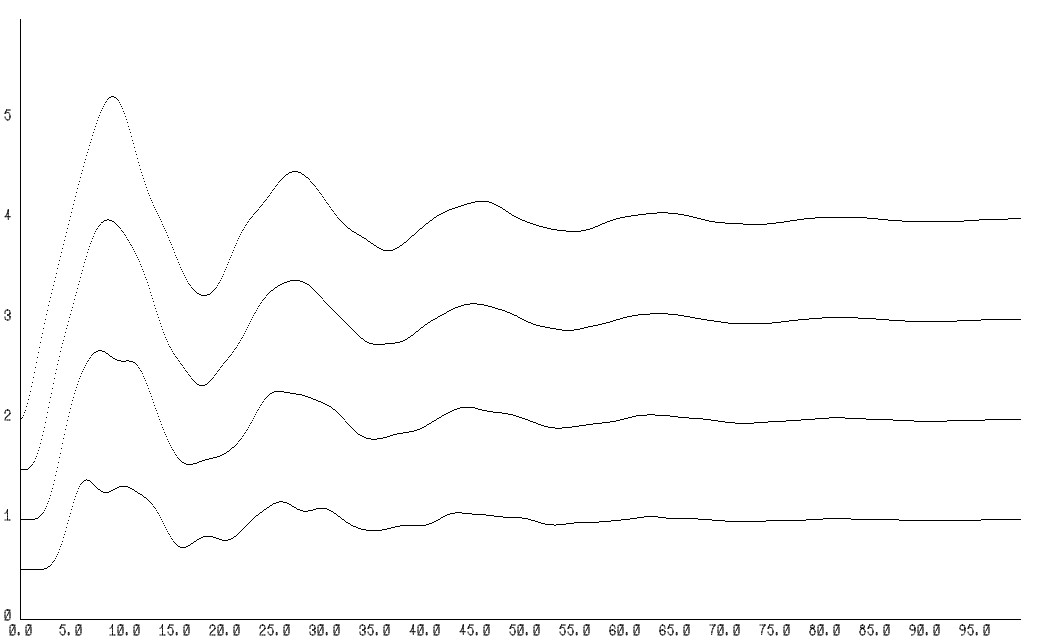
\includegraphics[width=8cm]{./springSys1D.jpg}
\end{center} 

\begin{center}
./springSys2Dk20.jpg\\
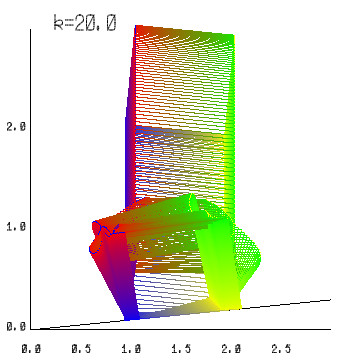
\includegraphics[width=8cm]{./springSys2Dk20.jpg}
\end{center} 
\newpage
\begin{center}
./springSys2Dk50.jpg\\
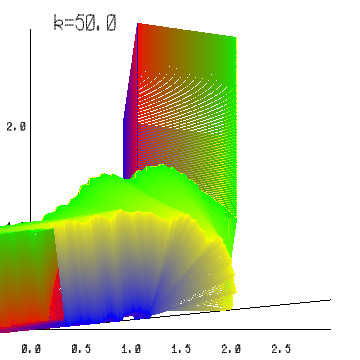
\includegraphics[width=8cm]{./springSys2Dk50.jpg}
\end{center} 

\begin{center}
./springSys2Dk100.jpg\\
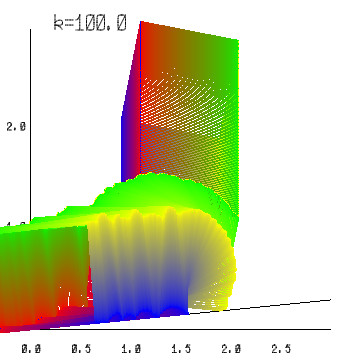
\includegraphics[width=8cm]{./springSys2Dk100.jpg}
\end{center} 
\newpage
\begin{center}
./springSys2Dk500.jpg\\
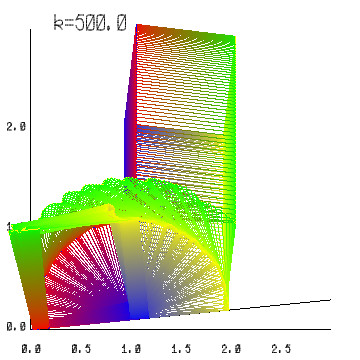
\includegraphics[width=8cm]{./springSys2Dk500.jpg}
\end{center} 

\begin{center}
./springSys2Dk1000.jpg\\
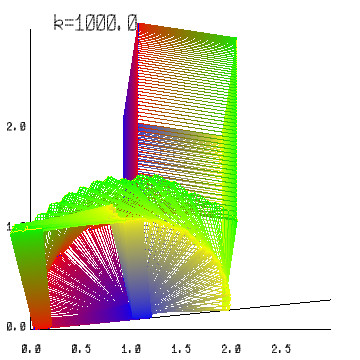
\includegraphics[width=8cm]{./springSys2Dk1000.jpg}
\end{center} 

\end{document}


